\documentclass[Lau,binding=0.6cm,oneside,noexaminfo]{sapthesis}
%\usepackage{hyperref}
\usepackage{microtype}
\usepackage[english]{babel}
\usepackage[utf8]{inputenx}
\usepackage{graphicx}
\usepackage{float} % Include the float package
\usepackage{skmath}
\usepackage{amsmath, xparse}
\usepackage{wrapfig}
\usepackage{float}
\usepackage{amsmath,amssymb}
\usepackage{sidecap}
\usepackage{xcolor}
\usepackage{gensymb}
\usepackage{caption}
\usepackage{tabularx}
\usepackage{geometry}
\usepackage{csvsimple}
\usepackage{subfig}
\usepackage{placeins}
\usepackage{xfrac}
\usepackage[makeroom]{cancel}
\usepackage{verbatim}
\usepackage{ gensymb }
\usepackage{ longtable }
\usepackage{geometry}
\usepackage{eucal}
%\usepackage{hyperref}
\usepackage{braket}
\usepackage{bbold}
\usepackage[hidelinks]{hyperref}
\hypersetup{pdftitle={Sapthesis class example},pdfauthor={Francesco Beccari}}

% Remove in a normal thesis
\usepackage{lipsum}
\usepackage{curve2e}
\definecolor{gray}{gray}{0.4}
\newcommand{\bs}{\textbackslash}

% Commands for the titlepage
\title{}
\author{}
\IDnumber{}
\course{Corso di Laurea Magistrale in Fisica}
\courseorganizer{Facoltà di Scienze Matematiche, Fisiche e Naturali}
\AcademicYear{}
\copyyear{}
\advisor{}
\coadvisor{}
\authoremail{}

%\examdate{16 April 2013}
%\examiner{Prof. Nome Cognome}
%\examiner{Prof. Nome Cognome}
%\examiner{Dr. Nome Cognome}
%\versiondate{\today}
\begin{document}

\frontmatter

\maketitle



%\begin{abstract}

%\end{abstract}

%\begin{acknowledgments}
    
%\end{acknowledgments}

\dedication{}


\newpage
\null
\thispagestyle{empty}
\newpage

\tableofcontents

% Do not use the starred version of the chapter command!


\newpage
\null
\thispagestyle{empty}
\newpage


\mainmatter

\chapter*{Introduction}
Le proteine rappresentano una classe di biomolecole essenziali alla vita, costituendo la base funzionale e strutturale di tutti gli organismi viventi. Composte da catene di amminoacidi connesse tramite legami peptidici, esse si distinguono per la loro capacità di assumere una straordinaria varietà di conformazioni tridimensionali. Questa caratteristica conferisce alle proteine una flessibilità funzionale senza precedenti, permettendo loro di partecipare a una vasta gamma di processi biologici.

Tra le principali funzioni delle proteine si annoverano:
\begin{itemize}
    \item \textbf{Catalisi enzimatica:} Le proteine enzimatiche accelerano le reazioni chimiche, riducendo l'energia di attivazione e regolando i processi metabolici cellulari.
    \item \textbf{Ruoli strutturali:} Alcune proteine, come il collagene o la cheratina, forniscono supporto meccanico e integrità strutturale ai tessuti.
    \item \textbf{Trasporto:} Molecole come l'emoglobina facilitano il trasporto di ossigeno, mentre altre proteine trasportano nutrienti e ioni attraverso le membrane cellulari.
    \item \textbf{Regolazione e segnalazione:} Le proteine svolgono ruoli chiave nella trasduzione dei segnali cellulari e nella regolazione dell'espressione genica.
\end{itemize}

Le proteine, dunque, sono sia i costruttori sia i regolatori della vita, operando con precisione nei vari contesti fisiologici.

\section*{Conformazioni proteiche e modi funzionali}
La struttura tridimensionale di una proteina è determinata dalla sequenza di amminoacidi (struttura primaria) e dalle interazioni chimiche che stabilizzano la struttura secondaria, terziaria e, in molti casi, quaternaria. Queste interazioni portano alla formazione di strutture funzionali in grado di riconoscere substrati specifici o interagire con altre molecole.

Un concetto fondamentale nello studio delle proteine è quello dei \emph{modi funzionali}, ovvero le configurazioni dinamiche che una proteina può assumere per adattarsi ai cambiamenti ambientali o alle interazioni con partner molecolari. Tali cambiamenti strutturali sono spesso descritti come un insieme di microstati energetici, ciascuno con una probabilità associata.

\section*{Distribuzioni di probabilità nelle proteine}
Le fluttuazioni strutturali delle proteine possono essere studiate in termini di distribuzioni di probabilità (Probability Density Functions, PDF). Una PDF descrive la probabilità di trovare una proteina in un dato stato conformazionale o con un certo valore di energia. Le proteine non sono statiche, ma vivono in un continuo dinamico tra diversi stati, ciascuno caratterizzato da una differente energia libera. 

L'analisi delle PDF trova applicazione in numerosi contesti, tra cui:
\begin{itemize}
    \item Studio della stabilità proteica e delle transizioni conformazionali.
    \item Descrizione dell'affinità di legame tra proteina e ligando.
    \item Modellizzazione dei processi di ripiegamento proteico (\emph{protein folding}).
\end{itemize}

\section*{Allostericità: una proprietà emergente delle proteine}

Un fenomeno straordinario legato alla dinamicità proteica è l’\emph{allostericità}, ovvero la capacità di una proteina di trasmettere un segnale o un cambiamento conformazionale da un sito all’altro. Questo meccanismo fondamentale consente a molte proteine di svolgere le loro funzioni biologiche in modo altamente regolato, rappresentando una chiave di volta per la comprensione della biochimica cellulare e per lo sviluppo di nuovi farmaci. L’allostericità gioca un ruolo cruciale nella regolazione dell’attività enzimatica, nella trasduzione del segnale e nella comunicazione intracellulare, fungendo da "interruttore molecolare" che risponde a stimoli ambientali e intracellulari.

\subsection*{Definizione e principi fondamentali dell’allostericità}
L’allostericità, dal greco \emph{allos} (altro) e \emph{stereos} (struttura), si riferisce a un fenomeno in cui l'interazione di una molecola (effettore) con un sito specifico di una proteina, noto come \emph{sito allosterico}, provoca una modifica conformazionale che influenza l'attività funzionale di un altro sito, solitamente il \emph{sito attivo}. Questo processo non avviene attraverso interazioni dirette tra i due siti, ma mediante cambiamenti nella rete di interazioni intramolecolari che regolano la struttura e la dinamica della proteina.

Dal punto di vista termodinamico, l’allostericità può essere descritta come una modulazione della distribuzione dei microstati energetici di una proteina. In altre parole, l’interazione con un effettore allosterico altera l’insieme degli stati conformazionali disponibili, facilitando o inibendo l’accesso a configurazioni funzionali. Questo fenomeno è stato osservato in numerose proteine chiave, tra cui l’emoglobina, che sfrutta l’allostericità per modulare il trasporto dell’ossigeno.

\subsection*{Modelli classici dell’allostericità}
I primi modelli teorici dell’allostericità sono stati introdotti per spiegare la cooperatività nell’emoglobina e in altri sistemi proteici. Due approcci fondamentali hanno dominato la comprensione del fenomeno:

\begin{itemize}
    \item \textbf{Modello concertato (MWC):} Proposto da Monod, Wyman e Changeux nel 1965, questo modello assume che una proteina allosterica esista in equilibrio tra due stati conformazionali principali, \emph{R} (relassato) e \emph{T} (teso), con l’effettore che stabilizza uno di questi stati. Tutte le subunità di una proteina oligomerica cambiano conformazione simultaneamente.
    \item \textbf{Modello sequenziale (KNF):} Introdotto da Koshland, Némethy e Filmer, questo modello suggerisce che il legame di un effettore a una subunità induca cambiamenti conformazionali locali, che a loro volta influenzano le subunità vicine in modo graduale e indipendente.
\end{itemize}

Entrambi i modelli hanno contribuito a chiarire i meccanismi di base dell’allostericità, sebbene studi successivi abbiano dimostrato che molti sistemi biologici mostrano caratteristiche che non rientrano completamente in uno dei due approcci.

\subsection*{Allostericità e dinamica proteica}
La moderna comprensione dell’allostericità si basa sempre più sull’idea che il fenomeno sia intrinsecamente legato alla dinamicità proteica. Le proteine non sono strutture rigide, ma ensemble di stati conformazionali che fluttuano su scale temporali e spaziali. Gli effettori allosterici alterano questa rete dinamica, rimodellando i percorsi energetici che collegano i vari stati funzionali.

\begin{figure}[h!]
    \centering
    \includegraphics[width=0.8\textwidth]{allostericity_dynamics.png}
    \caption{Rappresentazione schematica dell’allostericità: l’interazione con un effettore allosterico (sito A) induce un cambiamento conformazionale che influenza un sito distante (sito B).}
    \label{fig:allostericity}
\end{figure}

Questa visione dinamica si integra con approcci computazionali, come la dinamica molecolare e le reti di interazioni residue, che permettono di identificare percorsi specifici attraverso i quali l’informazione allosterica si propaga all’interno della proteina.

\subsection*{Esempi biologici di allostericità}
L’allostericità è presente in numerosi sistemi biologici, svolgendo funzioni essenziali in diversi contesti fisiologici:

\begin{itemize}
    \item \textbf{Emoglobina:} Uno degli esempi più noti, l’allostericità nell’emoglobina consente il rilascio cooperativo dell’ossigeno ai tessuti. Gli ioni H\(^+\) e il 2,3-bisfosfoglicerato agiscono come effettori negativi, stabilizzando lo stato T e favorendo il rilascio dell’ossigeno.
    \item \textbf{Recettori accoppiati a proteine G (GPCR):} Questi recettori trasducono segnali extracellulari attraverso meccanismi allosterici che coinvolgono cambiamenti conformazionali tra il dominio extracellulare e quello intracellulare.
    \item \textbf{Enzimi regolatori:} Molti enzimi, come l’aspartato transcarbamilasi, sono regolati allostericamente per coordinare le vie metaboliche in risposta ai bisogni cellulari.
\end{itemize}

\subsection*{Implicazioni biotecnologiche e farmacologiche}
L’allostericità rappresenta un obiettivo interessante per lo sviluppo di nuovi farmaci. Gli \emph{allosteric modulators} offrono diversi vantaggi rispetto agli inibitori o agonisti tradizionali:

\begin{itemize}
    \item \textbf{Selettività:} Gli effettori allosterici interagiscono con siti diversi da quelli conservati, riducendo il rischio di effetti collaterali.
    \item \textbf{Regolazione fine:} Possono modulare l’attività proteica in modo più sottile, senza bloccarla completamente.
    \item \textbf{Riduzione della resistenza:} Poiché il sito allosterico è meno soggetto a pressioni evolutive rispetto al sito attivo, è meno probabile che emergano mutazioni resistenti.
\end{itemize}

Esempi di farmaci allosterici già in uso includono modulatori per recettori GPCR, come i farmaci per il trattamento della schizofrenia e dell’asma.

\subsection*{Conclusioni}
L’allostericità è una proprietà emergente delle proteine che illustra la complessità e l’eleganza della regolazione molecolare nei sistemi biologici. Grazie alla combinazione di approcci sperimentali e computazionali, stiamo iniziando a comprendere meglio i meccanismi alla base di questo fenomeno, con promettenti applicazioni in campo medico e biotecnologico. Continuare a esplorare l’allostericità non solo ci aiuterà a rispondere a domande fondamentali sulla biologia molecolare, ma aprirà anche nuove strade per l’innovazione terapeutica.

\section*{La proteina PDZ: una panoramica}

La proteina PDZ rappresenta una delle classi più studiate di domini proteici modulari, essenziali per il mantenimento dell’organizzazione spaziale e funzionale nelle cellule. Il nome "PDZ" deriva dai primi tre membri della famiglia in cui è stato identificato: \emph{Post-synaptic density protein 95 (PSD-95)}, \emph{Discs large tumor suppressor (Dlg1)} e \emph{Zona occludens-1 (ZO-1)}. I domini PDZ sono fondamentali per la formazione di complessi multiproteici e per l’ancoraggio di proteine bersaglio a regioni specifiche della membrana cellulare.

\subsection*{Struttura e caratteristiche principali del dominio PDZ}

Il dominio PDZ è composto da circa 80-90 residui amminoacidici, che si organizzano in una struttura a barile $\beta$ (\emph{$\beta$-sandwich}) formata da sei filamenti $\beta$ alternati e due $\alpha$-eliche. Questa conformazione crea una tasca idrofobica specifica per il legame con i ligandi, tipicamente localizzati nelle regioni C-terminali delle proteine target.

Le caratteristiche principali del dominio PDZ includono:
\begin{itemize}
    \item \textbf{Specificità di legame:} Il dominio PDZ riconosce sequenze specifiche di 4-5 amminoacidi, note come \emph{motivi PDZ-binding}, situate alla fine delle proteine bersaglio.
    \item \textbf{Modularità:} I domini PDZ possono essere combinati in proteine più grandi, consentendo una vasta gamma di interazioni con altre proteine.
    \item \textbf{Versatilità funzionale:} Grazie alla loro struttura conservata e al riconoscimento sequenza-specifico, i domini PDZ partecipano a processi chiave come la segnalazione cellulare, l’organizzazione sinaptica e la polarità cellulare.
\end{itemize}

\subsection*{Funzioni biologiche del dominio PDZ}

I domini PDZ giocano un ruolo centrale in diversi processi biologici. Tra le loro funzioni principali si annoverano:

\subsubsection*{1. Organizzazione della segnalazione cellulare}
Il dominio PDZ funge da piattaforma di ancoraggio per i complessi proteici coinvolti nella trasduzione del segnale. Ad esempio, proteine PDZ come PSD-95 si associano ai recettori del glutammato nei neuroni, contribuendo alla formazione di sinapsi funzionali e alla modulazione della plasticità sinaptica.

\subsubsection*{2. Mantenimento della polarità cellulare}
Le proteine contenenti domini PDZ, come ZO-1 e Dlg1, sono fondamentali per mantenere la polarità apico-basolaterale nelle cellule epiteliali. Attraverso l’interazione con le giunzioni strette, queste proteine assicurano una corretta compartimentalizzazione delle membrane cellulari.

\subsubsection*{3. Traffico di proteine e membrana}
I domini PDZ regolano il trasporto intracellulare di proteine bersaglio verso compartimenti specifici. Un esempio è rappresentato dalla proteina NHERF1, che interagisce con il recettore della paratiroide per regolare il riassorbimento del calcio nei reni.

\subsubsection*{4. Sinapsi e plasticità neuronale}
Nei neuroni, i domini PDZ sono coinvolti nell’organizzazione delle proteine postsinaptiche. La formazione di complessi proteici attraverso interazioni PDZ-ligando è essenziale per la stabilizzazione dei recettori di membrana e per la trasmissione sinaptica efficace.

\subsection*{Il dominio PDZ e la dinamica allosterica}

Un aspetto emergente nello studio delle proteine PDZ è la loro capacità di esibire dinamiche allosteriche. Sebbene il dominio PDZ sia relativamente piccolo, presenta una notevole plasticità conformazionale che gli consente di rispondere a stimoli molecolari attraverso cambiamenti strutturali.

\subsubsection*{Meccanismo di allostericità}
L’allostericità nel dominio PDZ si manifesta quando il legame di un ligando nella tasca canonica induce modifiche conformazionali che influenzano la capacità di legare altri partner molecolari. Questo fenomeno è particolarmente evidente nei domini PDZ delle proteine multi-PDZ, dove l’interazione con un ligando può modulare la funzione di altri domini.

\subsubsection*{Implicazioni biologiche}
L’allostericità nei domini PDZ è cruciale per processi come:
\begin{itemize}
    \item \emph{Coordinazione sinaptica:} Le modifiche conformazionali nei domini PDZ di PSD-95 regolano l’associazione con recettori postsinaptici.
    \item \emph{Risposta a stimoli esterni:} Il dominio PDZ può agire come sensore molecolare, adattando la sua funzione a variazioni ambientali o fisiologiche.
\end{itemize}

\subsection*{Metodologie di studio del dominio PDZ}

Lo studio delle proteine PDZ ha beneficiato di un’ampia gamma di approcci sperimentali e computazionali:

\subsubsection*{1. Cristallografia a raggi X}
Le strutture cristallografiche hanno fornito informazioni dettagliate sulla tasca di legame e sulle interazioni ligando-dominio. Ad esempio, le strutture di PSD-95 e ZO-1 hanno rivelato l’importanza delle interazioni idrofobiche nel riconoscimento del ligando.

\subsubsection*{2. Risonanza magnetica nucleare (NMR)}
L’NMR ha permesso di osservare le dinamiche conformazionali del dominio PDZ in soluzione, evidenziando la presenza di microstati energetici correlati all’allostericità.

\subsubsection*{3. Simulazioni molecolari}
Le simulazioni molecolari hanno fornito una visione dettagliata dei processi dinamici del dominio PDZ, inclusi i meccanismi di legame e i cambiamenti conformazionali indotti.

\subsubsection*{4. Approcci sperimentali funzionali}
Mutagenesi sito-specifica e saggi funzionali sono stati utilizzati per identificare residui chiave per il legame del ligando e per testare l’impatto dell’allostericità sulla funzione proteica.

\subsection*{Implicazioni biomediche delle proteine PDZ}

Le proteine contenenti domini PDZ sono coinvolte in numerose patologie, tra cui:
\begin{itemize}
    \item \textbf{Tumori:} Alterazioni nelle interazioni PDZ-ligando possono contribuire alla perdita di polarità cellulare e alla progressione tumorale.
    \item \textbf{Malattie neurodegenerative:} Le disfunzioni nei complessi PDZ sono associate a patologie come la malattia di Alzheimer, dove la segnalazione sinaptica è compromessa.
    \item \textbf{Malattie cardiovascolari:} Domini PDZ regolano i canali ionici e i recettori coinvolti nel controllo della pressione sanguigna e nella contrattilità cardiaca.
\end{itemize}

\subsection*{Conclusioni}

Il dominio PDZ rappresenta un modello ideale per studiare le interazioni proteina-proteina e i meccanismi allosterici alla base delle funzioni cellulari. La sua modularità, specificità di legame e versatilità funzionale lo rendono un bersaglio fondamentale per lo sviluppo di terapie innovative volte a modulare l’attività proteica in contesti patologici.
\chapter{Modi normali nelle proteine}

\section*{Introduzione ai modi normali}
La teoria dei modi normali (Normal Mode Analysis, NMA) è una tecnica fondamentale per analizzare le fluttuazioni dinamiche delle proteine a livello atomico. Questa metodologia consente di studiare le oscillazioni collettive delle strutture tridimensionali delle proteine attorno a uno stato di equilibrio, modellando il sistema come una rete di oscillatori armonici. I modi normali rappresentano i movimenti collettivi indipendenti che compongono la dinamica della proteina.

Matematicamente, la teoria dei modi normali si basa sull'approssimazione di un minimo locale della superficie di energia potenziale. In questa sezione, verrà introdotto il formalismo matematico alla base dell'NMA, con esempi applicati alla dinamica delle proteine.

\section{Modello matematico dei modi normali}

\subsection*{1. Energia potenziale della proteina}
L'energia potenziale di una proteina può essere descritta come una funzione $V(\mathbf{x})$, dove $\mathbf{x} = (x_1, x_2, \dots, x_{3N})$ rappresenta le coordinate dei $N$ atomi nella struttura tridimensionale. In prossimità di un minimo locale, l'energia può essere approssimata tramite uno sviluppo di Taylor di secondo ordine:
\[
V(\mathbf{x}) \approx V(\mathbf{x}_0) + \frac{1}{2} \sum_{i,j} \frac{\partial^2 V}{\partial x_i \partial x_j} \Delta x_i \Delta x_j,
\]
dove $\mathbf{x}_0$ è la configurazione di equilibrio e $\Delta \mathbf{x} = \mathbf{x} - \mathbf{x}_0$ rappresenta la deviazione rispetto all'equilibrio. Il termine $\frac{\partial^2 V}{\partial x_i \partial x_j}$ definisce la matrice hessiana $\mathbf{H}$ dell'energia potenziale:
\[
\mathbf{H} = \begin{bmatrix}
\frac{\partial^2 V}{\partial x_1^2} & \frac{\partial^2 V}{\partial x_1 \partial x_2} & \cdots & \frac{\partial^2 V}{\partial x_1 \partial x_{3N}} \\
\frac{\partial^2 V}{\partial x_2 \partial x_1} & \frac{\partial^2 V}{\partial x_2^2} & \cdots & \frac{\partial^2 V}{\partial x_2 \partial x_{3N}} \\
\vdots & \vdots & \ddots & \vdots \\
\frac{\partial^2 V}{\partial x_{3N} \partial x_1} & \frac{\partial^2 V}{\partial x_{3N} \partial x_2} & \cdots & \frac{\partial^2 V}{\partial x_{3N}^2}
\end{bmatrix}.
\]

\subsection*{2. Risoluzione del problema agli autovalori}
Il movimento della proteina può essere descritto tramite la seconda legge di Newton:
\[
M \frac{d^2 \mathbf{x}}{dt^2} = -\mathbf{H} \Delta \mathbf{x},
\]
dove $M$ è una matrice diagonale che contiene le masse atomiche. Dividendo per $M$ e trasformando il sistema in coordinate ridotte, si ottiene l'equazione del moto:
\[
\frac{d^2 \mathbf{q}}{dt^2} = -\mathbf{H}' \mathbf{q},
\]
dove $\mathbf{H}' = M^{-1/2} \mathbf{H} M^{-1/2}$ è la matrice hessiana ridotta. La soluzione di questo sistema si ottiene diagonalizzando $\mathbf{H}'$:
\[
\mathbf{H}' \mathbf{v}_i = \lambda_i \mathbf{v}_i,
\]
dove $\lambda_i$ sono gli autovalori (frequenze quadratiche dei modi normali) e $\mathbf{v}_i$ sono gli autovettori (i modi normali).

\section{Interpretazione fisica dei modi normali}

Gli autovalori $\lambda_i$ rappresentano le frequenze quadratiche associate ai modi normali, mentre gli autovettori $\mathbf{v}_i$ descrivono la direzione del movimento per ciascun modo. I modi normali con autovalori piccoli (basse frequenze) corrispondono a movimenti collettivi lenti e di grande ampiezza, spesso associati a processi funzionali delle proteine, come l'apertura e chiusura di tasche enzimatiche o il movimento di domini.

\subsection*{1. Modi rigidi e vibrazionali}
I primi sei modi normali, corrispondenti agli spostamenti traslazionali e rotazionali rigidi della proteina, hanno autovalori nulli o prossimi allo zero. Gli altri modi descrivono oscillazioni vibrazionali interne della proteina.

\subsection*{2. Fluttuazioni termiche}
Le fluttuazioni termiche di una proteina possono essere descritte utilizzando i modi normali. La deviazione media quadratica di un atomo $i$ in equilibrio è proporzionale all'inverso degli autovalori:
\[
\langle (\Delta x_i)^2 \rangle \propto \sum_{k} \frac{(v_k)_i^2}{\lambda_k},
\]
dove $(v_k)_i$ è la componente del $k$-esimo autovettore associata all’atomo $i$.

\section{Applicazioni della teoria dei modi normali alle proteine}

\subsection*{1. Analisi della dinamica funzionale}
La teoria dei modi normali è stata utilizzata per comprendere i movimenti collettivi delle proteine, come l’apertura e la chiusura delle tasche enzimatiche. Ad esempio, per l'enzima adenilato ciclasi, i modi normali a basse frequenze mostrano oscillazioni che facilitano l'accesso del substrato al sito attivo.

\subsection*{2. Calcolo dei fattori B}
I fattori B, osservati nella cristallografia a raggi X, rappresentano la flessibilità atomica in una struttura proteica. Tramite NMA, è possibile prevedere i fattori B teorici:
\[
B_i = \frac{8 \pi^2}{3} \langle (\Delta x_i)^2 \rangle.
\]

\subsection*{3. Disegno di farmaci}
La dinamica delle proteine, studiata tramite NMA, è essenziale per il design di farmaci. I movimenti lenti e collettivi identificati tramite modi normali possono rivelare siti allosterici potenziali per l’intervento farmacologico.

\subsection*{4. Stabilità e ripiegamento proteico}
I modi normali possono essere utilizzati per studiare il ripiegamento proteico e le transizioni conformazionali. Ad esempio, analizzando le frequenze dei modi, è possibile identificare i movimenti correlati alla destabilizzazione di strutture secondarie.

\section{Modelli semplificati: elastic network model (ENM)}

Per ridurre la complessità computazionale, sono stati sviluppati modelli semplificati come l’Elastic Network Model (ENM). In questi modelli, gli atomi della proteina sono rappresentati come nodi connessi da molle, e l’energia potenziale è descritta come:
\[
V = \frac{1}{2} \sum_{i<j} k_{ij} (d_{ij} - d_{ij}^0)^2,
\]
dove $d_{ij}$ è la distanza tra gli atomi $i$ e $j$, $d_{ij}^0$ è la distanza di equilibrio, e $k_{ij}$ è la costante elastica.

L’ENM semplifica il calcolo della matrice hessiana, rendendo l’analisi dei modi normali computazionalmente più efficiente.

\section{Conclusioni}
La teoria dei modi normali offre una descrizione dettagliata delle dinamiche proteiche, fornendo informazioni preziose sui movimenti collettivi e sulle fluttuazioni termiche. Applicata a contesti biologici, come il design di farmaci e lo studio della funzione enzimatica, l'NMA rappresenta uno strumento potente per comprendere il comportamento dinamico delle proteine.
\chapter{Gaussian Network Models (GNM) nelle proteine}

\section*{Introduzione ai modelli di rete gaussiani}
Il Gaussian Network Model (GNM) è un approccio semplificato ma efficace per analizzare le dinamiche collettive delle proteine basandosi sulla loro struttura tridimensionale. Questo modello si colloca nella categoria degli \textit{elastic network models} (ENM) e rappresenta una potente astrazione per descrivere le fluttuazioni attorno alla configurazione nativa di una proteina. Per costruire una descrizione rigorosa, è essenziale passare da una rappresentazione generale della dinamica molecolare, basata sull'Hamiltoniana, a un sistema equivalente che utilizza molle armoniche per modellare le interazioni tra i residui.

\section{Dall’Hamiltoniana alla descrizione elastica}
La dinamica completa di una proteina può essere rappresentata da un'Hamiltoniana generica, che descrive l'energia totale del sistema come somma dell'energia cinetica e dell'energia potenziale:

\begin{equation}
H = T + V,
\end{equation}

dove $T$ rappresenta l'energia cinetica e $V$ l'energia potenziale. Nello specifico, l'energia cinetica è espressa come:

\begin{equation}
T = \frac{1}{2} \sum_{i=1}^{N} m_i \|\dot{\mathbf{r}}_i\|^2,
\end{equation}

con $m_i$ massa del residuo $i$, $\dot{\mathbf{r}}_i$ velocità del residuo $i$, e $N$ il numero totale di residui. L'energia potenziale $V$ descrive le interazioni tra i residui e, in linea di principio, include termini complessi che considerano legami covalenti, interazioni non covalenti e forze di esclusione sterica.

\subsection*{Semplificazione tramite approccio armonico}
Per studiare le fluttuazioni attorno alla configurazione nativa, si assume che le deviazioni dalle posizioni di equilibrio siano piccole. In questo regime, l'energia potenziale può essere approssimata tramite un'espansione di Taylor al secondo ordine attorno alla configurazione nativa $\{\mathbf{r}_i^0\}$:

\begin{equation}
V(\{\mathbf{r}_i\}) \approx V_0 + \frac{1}{2} \sum_{i,j=1}^N \frac{\partial^2 V}{\partial \mathbf{r}_i \partial \mathbf{r}_j} \Delta \mathbf{r}_i \cdot \Delta \mathbf{r}_j,
\end{equation}

dove $V_0$ è il valore dell'energia potenziale nella configurazione nativa e $\Delta \mathbf{r}_i = \mathbf{r}_i - \mathbf{r}_i^0$ rappresenta la deviazione della posizione del residuo $i$ rispetto all'equilibrio. Il termine di ordine zero può essere ignorato poiché non contribuisce alla dinamica, e il termine di ordine uno si annulla poiché la forza è nulla all'equilibrio. Pertanto, l'energia potenziale è dominata dal termine quadratico.

La matrice delle seconde derivate, detta matrice Hessiana $\mathbf{H}$, cattura la curvatura locale dell'energia potenziale:

\begin{equation}
H_{ij} = \frac{\partial^2 V}{\partial \mathbf{r}_i \partial \mathbf{r}_j}.
\end{equation}

\subsection*{Modello a molle armoniche}
In un GNM, l'Hamiltoniana viene ulteriormente semplificata assumendo che i residui siano collegati da molle armoniche, con una costante elastica uniforme $\gamma$. In questo modello, l'energia potenziale è scritta come:

\begin{equation}
V(\{\Delta \mathbf{r}_i\}) = \frac{\gamma}{2} \sum_{i=1}^N \sum_{j=1}^N \Gamma_{ij} (\Delta \mathbf{r}_i \cdot \Delta \mathbf{r}_j),
\end{equation}

dove $\mathbf{\Gamma}$ è la matrice di Kirchoff, definita come:

\begin{equation}
\Gamma_{ij} =
\begin{cases}
-1 & \text{se } r_{ij} \leq R_c \text{ e } i \neq j, \\
\sum_{k \neq i} A_{ik} & \text{se } i = j,
\end{cases}
\end{equation}

e $A_{ij}$ è la matrice di adiacenza della rete, che rappresenta le connessioni elastiche tra i residui basate su un cutoff di distanza $R_c$:

\begin{equation}
A_{ij} =
\begin{cases}
1 & \text{se } r_{ij} \leq R_c \text{ e } i \neq j, \\
0 & \text{altrimenti.}
\end{cases}
\end{equation}

In questo contesto, $\gamma$ rappresenta una costante elastica uniforme che caratterizza la rigidità delle molle.

\subsection*{Energia totale del sistema}
L'Hamiltoniana finale, che combina l'energia cinetica e quella potenziale armonica, è quindi data da:

\begin{equation}
H = \frac{1}{2} \sum_{i=1}^N m_i \|\dot{\mathbf{r}}_i\|^2 + \frac{\gamma}{2} \sum_{i=1}^N \sum_{j=1}^N \Gamma_{ij} (\Delta \mathbf{r}_i \cdot \Delta \mathbf{r}_j).
\end{equation}

Questa forma descrive completamente il sistema in termini di una rete elastica di nodi (i residui) connessi da molle (le interazioni elastiche). Le equazioni del moto derivate da questa Hamiltoniana permettono di calcolare le fluttuazioni dinamiche e le correlazioni tra i residui.

\section{Fluttuazioni e correlazioni dinamiche}
Le fluttuazioni medie quadratiche $\langle (\Delta R_i)^2 \rangle$ di ciascun residuo e le correlazioni $\langle \Delta \mathbf{R}_i \cdot \Delta \mathbf{R}_j \rangle$ tra coppie di residui sono direttamente ottenibili risolvendo le equazioni di equilibrio. La matrice inversa di $\mathbf{\Gamma}$, detta \textit{matrice delle correlazioni inverse}, è fondamentale per queste analisi:

\begin{equation}
\langle \Delta \mathbf{R} \Delta \mathbf{R}^T \rangle \propto \mathbf{\Gamma}^{-1}.
\end{equation}

Le fluttuazioni medie quadratiche per un residuo $i$ sono date da:

\begin{equation}
\langle (\Delta R_i)^2 \rangle = \left[ \mathbf{\Gamma}^{-1} \right]_{ii},
\end{equation}

mentre le correlazioni tra i residui $i$ e $j$ sono:

\begin{equation}
\langle \Delta R_i \cdot \Delta R_j \rangle = -\left[ \mathbf{\Gamma}^{-1} \right]_{ij}.
\end{equation}
\section{Conclusioni}
Gli indicatori dinamici, come la correlazione, la risposta lineare e l’entropia di produzione, forniscono strumenti matematici potenti per analizzare i meccanismi allosterici delle proteine. Combinando questi approcci, è possibile ottenere una comprensione dettagliata delle reti dinamiche che governano la funzione proteica, aprendo nuove prospettive per la progettazione di farmaci e per l'ingegneria delle proteine.


\chapter{Indicatori per l'analisi delle dinamiche proteiche e allosteriche}
\subsection{Il concetto di indicatori dinamici}

Gli indicatori dinamici rappresentano strumenti matematici e fisici fondamentali per analizzare e caratterizzare le proprietà dinamiche di sistemi complessi, come le proteine, le reti molecolari o altri sistemi biologici. Essi si basano su una descrizione approfondita delle fluttuazioni, delle interazioni e dei processi stocastici che governano il comportamento collettivo dei componenti del sistema. L'importanza degli indicatori dinamici risiede nella loro capacità di estrarre informazioni quantitative dalle dinamiche sottostanti, fornendo un quadro dettagliato delle relazioni tra struttura e funzione.

\paragraph{Definizione generale e motivazioni}
Gli indicatori dinamici sono definiti come quantità matematiche o fisiche che catturano aspetti specifici delle dinamiche di un sistema. A differenza delle analisi statiche, che considerano una singola configurazione della proteina o una struttura cristallografica, questi strumenti forniscono informazioni sulle fluttuazioni temporali, sui moti collettivi e sulle interazioni spaziali tra diverse parti del sistema.

In particolare, essi sono utili per:
\begin{itemize}
    \item \textbf{Quantificare le fluttuazioni locali e globali}: Le proteine non sono strutture rigide, ma oscillano costantemente attorno alla loro configurazione nativa a causa delle fluttuazioni termiche. Gli indicatori dinamici permettono di misurare e caratterizzare l'ampiezza di queste fluttuazioni, evidenziando regioni flessibili o rigidamente vincolate.
    \item \textbf{Esplorare le correlazioni dinamiche}: I residui all'interno di una proteina possono muoversi in modo sincronizzato o indipendente. Gli indicatori dinamici aiutano a determinare il grado di cooperazione tra questi movimenti, identificando moti collettivi che possono essere cruciali per la funzione biologica.
    \item \textbf{Valutare la trasmissione di informazioni}: Le proteine spesso trasmettono segnali conformazionali da una regione all'altra, un fenomeno noto come allostericità. Gli indicatori dinamici forniscono strumenti per quantificare il trasferimento di informazioni dinamiche attraverso la struttura proteica.
\end{itemize}

\paragraph{Fluttuazioni locali e globali: una panoramica}
Le fluttuazioni dinamiche di una proteina possono essere analizzate a diversi livelli di dettaglio:
\begin{itemize}
    \item \textbf{Fluttuazioni locali}: Queste descrivono i moti di piccoli gruppi di atomi o residui. Indicatori come le fluttuazioni medie quadratiche ($\langle (\Delta R_i)^2 \rangle$) forniscono una misura della mobilità di ciascun residuo, mettendo in evidenza le regioni flessibili come loop o terminali liberi.
    \item \textbf{Fluttuazioni globali}: Questi moti coinvolgono interi domini o subunità della proteina. Gli indicatori dinamici, come i modi normali a basse frequenze, permettono di identificare movimenti collettivi che supportano funzioni biologiche chiave, come l'apertura e chiusura di tasche enzimatiche.
\end{itemize}

\paragraph{Correlazioni dinamiche e interazioni tra residui}
Le correlazioni dinamiche rappresentano un altro aspetto critico delle dinamiche proteiche. Queste misurano il grado di sincronia nei movimenti di due residui o regioni distinte. Indicatori come la matrice delle correlazioni dinamiche $C_{ij}(t)$ sono fondamentali per:
\begin{itemize}
    \item Identificare reti di residui cooperativi, che spesso formano il cuore dei meccanismi allosterici.
    \item Distinguere tra movimenti sincroni (correlazioni positive) e movimenti opposti (anticorrelazioni negative).
\end{itemize}
Questi concetti sono particolarmente rilevanti per analizzare proteine multidominio, dove il coordinamento tra diversi segmenti è essenziale per la funzione.

\paragraph{Trasferimento di informazione e comunicazione dinamica}
Un ulteriore elemento chiave degli indicatori dinamici è la loro capacità di quantificare il trasferimento di informazioni tra diverse parti della proteina. Questo è cruciale per comprendere i meccanismi allosterici, in cui eventi locali, come il legame di un ligando, causano cambiamenti conformazionali che si propagano attraverso la struttura. Indicatori come la \textit{transfer entropy} ($TE$) permettono di:
\begin{itemize}
    \item Quantificare il flusso di informazione da un residuo a un altro.
    \item Identificare i "nodi" critici della rete dinamica che mediano la comunicazione tra regioni distanti.
\end{itemize}

\paragraph{Connessione con i processi stocastici}
Il comportamento dinamico di una proteina è governato da processi stocastici, che combinano forze deterministiche, come quelle elastiche, e fluttuazioni casuali termiche. Gli indicatori dinamici sono strettamente legati a questa descrizione probabilistica, poiché derivano da equazioni del moto che incorporano:
\begin{itemize}
    \item \textbf{Fluttuazioni termiche}: Modellate come rumore bianco gaussiano.
    \item \textbf{Reti elastiche}: Che descrivono le interazioni tra i residui vicini.
\end{itemize}
Questo quadro matematico consente di collegare gli indicatori dinamici a grandezze fisiche misurabili, come i fattori di Debye-Waller ($B$-factors) ottenuti dalla cristallografia a raggi X.

\paragraph{Relazione con le proprietà spettrali della matrice di Kirchhoff}
Un aspetto cruciale degli indicatori dinamici è la loro relazione con le proprietà spettrali della matrice di Kirchhoff, che descrive la connettività elastica del sistema. Gli autovalori $\lambda_k$ e gli autovettori $\mathbf{u}_k$ della matrice di Kirchhoff permettono di decomporre i movimenti dinamici in \textit{modi normali}, ciascuno caratterizzato da una frequenza e un'ampiezza specifica. Gli indicatori dinamici possono quindi essere interpretati come combinazioni ponderate di questi modi normali, fornendo una comprensione più profonda delle dinamiche collettive.

\paragraph{Applicazioni pratiche degli indicatori dinamici}
Gli indicatori dinamici sono stati applicati con successo in numerosi studi per:
\begin{itemize}
    \item Identificare regioni flessibili o rigide in enzimi, che sono spesso correlate a siti attivi o di legame.
    \item Analizzare i meccanismi di apertura e chiusura di canali ionici.
    \item Progettare proteine ingegnerizzate con proprietà dinamiche desiderate.
    \item Sviluppare farmaci mirati contro regioni funzionali identificate dinamicamente.
\end{itemize}

\paragraph{Limiti e sfide}
Nonostante il loro successo, gli indicatori dinamici presentano alcune limitazioni:
\begin{itemize}
    \item La loro interpretazione dipende fortemente dal modello utilizzato per descrivere la dinamica proteica (es. rete elastica vs dinamica molecolare).
    \item Alcuni indicatori richiedono una grande quantità di dati o calcoli intensivi, specialmente in sistemi complessi o di grandi dimensioni.
    \item La scelta dei parametri (es. cutoff di distanza, costanti elastiche) può influenzare significativamente i risultati.
\end{itemize}

\paragraph{Conclusioni}
Gli indicatori dinamici offrono un potente set di strumenti per analizzare le dinamiche proteiche, fornendo informazioni critiche sulle interazioni e sui meccanismi funzionali. La loro combinazione con modelli computazionali avanzati e dati sperimentali rappresenta una direzione promettente per future ricerche in biologia strutturale e biofisica.






\subsection{Tipologie di indicatori dinamici}

Nel contesto delle dinamiche proteiche, gli indicatori dinamici rappresentano strumenti essenziali per quantificare e comprendere i moti collettivi e locali di una proteina, analizzando non solo le interazioni statiche ma anche quelle temporali e causali. Questi indicatori consentono di esplorare le relazioni tra struttura, dinamica e funzione, fornendo informazioni fondamentali su come le proteine rispondono a stimoli interni o esterni e su come comunicano all'interno della loro rete molecolare.

\paragraph{Il ruolo degli indicatori dinamici nelle proteine}
Gli indicatori dinamici sono progettati per catturare diversi aspetti delle fluttuazioni e delle interazioni proteiche:
\begin{itemize}
    \item \textbf{Aspetto locale}: caratterizzano il comportamento di singoli residui o piccoli gruppi di residui.
    \item \textbf{Aspetto collettivo}: descrivono i moti che coinvolgono regioni più ampie della proteina o addirittura l'intera struttura.
    \item \textbf{Causalità}: determinano in che misura il movimento di una parte della proteina influenzi direttamente un'altra.
    \item \textbf{Allostericità}: identificano come le modifiche locali (ad esempio, il legame con un ligando) si traducano in cambiamenti funzionali globali.
\end{itemize}

La classificazione degli indicatori dinamici è utile per separare le informazioni relative ai diversi livelli di organizzazione della dinamica proteica. Nel contesto delle reti elastiche e delle descrizioni stocastiche, possiamo identificare tre categorie principali di indicatori dinamici: \textbf{correlazioni dinamiche}, \textbf{risposta lineare} e \textbf{trasferimento di informazione}. Ognuno di essi ha un ruolo specifico nella comprensione della dinamica proteica.

\subsubsection*{1. Correlazioni dinamiche}
Le correlazioni dinamiche rappresentano la sincronia nei movimenti di coppie di residui e sono descritte matematicamente dalla matrice delle correlazioni temporali $C_{ij}(t)$:
\begin{equation}
C_{ij}(t) = \langle x_i(0) x_j(t) \rangle,
\end{equation}
dove $x_i(t)$ e $x_j(t)$ rappresentano i movimenti dei residui $i$ e $j$ nel tempo, e $\langle \cdot \rangle$ denota la media sull’ensemble. Le correlazioni dinamiche hanno diverse interpretazioni:
\begin{itemize}
    \item \textbf{Correlazioni positive}: indicano che i residui si muovono in modo cooperativo nella stessa direzione.
    \item \textbf{Correlazioni negative}: rappresentano movimenti opposti, spesso associati a cambiamenti conformazionali significativi.
    \item \textbf{Correlazioni nulle}: suggeriscono che i movimenti di due residui sono indipendenti.
\end{itemize}

Le correlazioni dinamiche sono particolarmente utili per identificare \textit{reti di residui cooperativi}, che sono spesso coinvolte in meccanismi funzionali chiave come l'allostericità. Ad esempio, le correlazioni elevate tra un sito attivo e un sito distante possono indicare la presenza di un canale di comunicazione dinamico che trasmette segnali conformazionali attraverso la proteina.

\paragraph{Esempi applicativi delle correlazioni dinamiche}
Le correlazioni dinamiche sono state utilizzate per analizzare enzimi come l'HIV-1 proteasi, dove le correlazioni tra i flap e il core enzimatico hanno rivelato meccanismi di apertura e chiusura essenziali per la catalisi. Analogamente, nei canali ionici, le correlazioni dinamiche hanno permesso di identificare residui critici per la regolazione del flusso ionico.

\subsubsection*{2. Risposta lineare}
La risposta lineare misura come un residuo risponde a perturbazioni esterne applicate ad altri residui. Formalmente, la risposta dinamica è definita come:
\begin{equation}
R_{ij}(t) = \frac{\delta \langle x_i(t) \rangle}{\delta F_j(0)},
\end{equation}
dove $F_j(0)$ rappresenta una forza esterna applicata al residuo $j$ al tempo iniziale.

La risposta lineare è un indicatore di \textit{sensibilità dinamica}: descrive la misura in cui un residuo è influenzato dai cambiamenti in altre parti della proteina. In particolare, permette di identificare residui che agiscono come nodi critici nella rete di comunicazione interna della proteina.

\paragraph{Interpretazione fisica della risposta lineare}
La risposta $R_{ij}(t)$ è strettamente legata alla matrice di Kirchhoff $\mathbf{K}$ e ai suoi autovalori/autovettori. I residui che mostrano una risposta elevata a perturbazioni esterne sono spesso coinvolti in meccanismi di trasmissione del segnale. Inoltre:
\begin{itemize}
    \item Una risposta alta suggerisce una connessione dinamica forte tra due residui.
    \item Una risposta bassa implica una connessione debole o un’assenza di comunicazione diretta.
\end{itemize}

\paragraph{Utilizzo della risposta lineare nell'allostericità}
Nei sistemi allosterici, la risposta lineare può essere utilizzata per prevedere quali residui trasmettono segnali conformazionali dal sito di legame all'intera proteina. Ad esempio, in una proteina come l’emoglobina, la risposta lineare permette di mappare il percorso dinamico attraverso cui il legame dell’ossigeno in un sito attivo induce cambiamenti strutturali cooperativi.

\subsubsection*{3. Trasferimento di informazione}
Il trasferimento di informazione è un indicatore fondamentale per quantificare la causalità nelle dinamiche proteiche. Formalmente, si basa sulla misura di \textit{transfer entropy} (TE), definita come:
\begin{equation}
TE_{j \to i}(t) = \left\langle \log \frac{P[x_i(t) | x_i(0), x_j(0)]}{P[x_i(t) | x_i(0)]} \right\rangle,
\end{equation}
dove $P[x_i(t) | x_i(0), x_j(0)]$ è la probabilità condizionata del movimento del residuo $i$ dato lo stato iniziale di $i$ e $j$, e $P[x_i(t) | x_i(0)]$ esclude l’influenza di $j$.

\paragraph{Causalità e comunicazione dinamica}
A differenza delle correlazioni, che descrivono solo sincronia, il trasferimento di informazione identifica relazioni causali tra residui. Un valore elevato di $TE_{j \to i}(t)$ implica che i movimenti del residuo $j$ influenzano direttamente i movimenti del residuo $i$. Questo è cruciale per comprendere come le proteine trasmettono segnali conformazionali attraverso reti di interazioni dinamiche.

\paragraph{Importanza nell'allostericità}
Nel contesto dell'allostericità, il trasferimento di informazione permette di tracciare i percorsi dinamici che collegano un evento locale (come il legame di un ligando) a cambiamenti globali nella struttura proteica. Ad esempio:
\begin{itemize}
    \item Nelle chinasi, il trasferimento di informazione può rivelare come il legame di ATP regoli l'attività catalitica attraverso moti cooperativi.
    \item Nei recettori accoppiati a proteine G (GPCR), l’analisi del trasferimento di informazione evidenzia i residui chiave coinvolti nella trasduzione del segnale attraverso la membrana.
\end{itemize}

\paragraph{Calcolo e applicazione pratica}
Il calcolo del trasferimento di informazione si basa sull'analisi di traiettorie stocastiche e richiede una buona conoscenza delle proprietà dinamiche del sistema. È stato applicato con successo per identificare regioni allosteriche in numerosi sistemi proteici, aiutando a progettare farmaci che mirano a residui specifici per modulare la funzione proteica.

\paragraph{Conclusioni}
Le tre tipologie principali di indicatori dinamici – correlazioni dinamiche, risposta lineare e trasferimento di informazione – forniscono una gamma completa di strumenti per analizzare le dinamiche proteiche. Ciascuno di essi contribuisce a un aspetto specifico della comprensione delle relazioni dinamiche e causali nelle proteine, con applicazioni dirette nella biologia strutturale, nell'ingegneria proteica e nel design di farmaci. La loro combinazione offre una visione dettagliata e multilivello delle interazioni che governano i processi biologici.









\subsection{Gli indicatori dinamici come strumenti per lo studio delle proteine}
Gli indicatori dinamici sono definiti come quantità matematiche o fisiche che descrivono le proprietà dinamiche di un sistema complesso. Nel contesto delle proteine, questi indicatori aiutano a:
\begin{itemize}
    \item Quantificare le fluttuazioni dei residui attorno alla loro configurazione di equilibrio.
    \item Esplorare le correlazioni nei movimenti collettivi di residui distanti.
    \item Valutare la trasmissione di segnali conformazionali lungo la catena proteica.
\end{itemize}
Tali informazioni sono essenziali per comprendere fenomeni complessi come l’allostericità, in cui eventi locali, come il legame di un ligando, influenzano la dinamica e la funzione globale della proteina.

\subsection{Contesto generale: reti elastiche e modelli stocastici}
La modellazione dinamica delle proteine avviene solitamente tramite una rappresentazione semplificata: le reti elastiche. In questi modelli, una proteina è rappresentata come un grafo non orientato, in cui:
\begin{itemize}
    \item I nodi corrispondono a residui (o atomi specifici, come i $C_\alpha$).
    \item Gli spigoli rappresentano le connessioni elastiche tra residui, che possono essere determinate da un criterio di distanza (cutoff) o da interazioni chimiche specifiche.
\end{itemize}

La dinamica del sistema è poi descritta utilizzando equazioni differenziali stocastiche, che rappresentano la combinazione di forze deterministiche (elastiche) e fluttuazioni casuali (termiche). Queste equazioni consentono di calcolare quantità osservabili come:
\begin{itemize}
    \item \textbf{Correlazioni dinamiche}: la sincronia nei movimenti di coppie di residui.
    \item \textbf{Risposta lineare}: la sensibilità del sistema a piccole perturbazioni.
    \item \textbf{Trasferimento di informazione}: il flusso di dati dinamici tra residui distanti.
\end{itemize}

\subsection{Importanza degli indicatori dinamici nello studio delle proteine}
Lo studio delle dinamiche proteiche con indicatori dinamici ha portato a importanti scoperte in biofisica e biologia strutturale, come:
\begin{itemize}
    \item Identificazione di regioni altamente flessibili, che spesso corrispondono a loop o a terminali liberi.
    \item Individuazione di siti chiave responsabili della comunicazione allosterica.
    \item Interpretazione dei movimenti collettivi che supportano funzioni biologiche specifiche, come l’apertura e la chiusura di siti catalitici.
\end{itemize}
La capacità di quantificare tali proprietà è fondamentale per applicazioni come il design di farmaci e la progettazione di proteine.

\section{Modello matematico delle dinamiche proteiche}

\subsection{Rappresentazione di una proteina come rete elastica}
Un approccio comune per modellare le dinamiche proteiche è rappresentare la proteina come un grafo in cui i nodi corrispondono ai residui e gli spigoli descrivono interazioni elastiche. Questa rappresentazione semplificata cattura efficacemente i moti collettivi che sono rilevanti per la funzione.

La rete è costruita considerando un cutoff di distanza $R_c$:
\begin{equation}
r_{ij} = \|\mathbf{r}_i - \mathbf{r}_j\| \leq R_c,
\end{equation}
dove $r_{ij}$ è la distanza tra i residui $i$ e $j$. Questo criterio crea una matrice di adiacenza $\mathbf{A}$, con elementi:
\begin{equation}
A_{ij} =
\begin{cases}
1 & \text{se } r_{ij} \leq R_c \text{ e } i \neq j, \\
0 & \text{altrimenti.}
\end{cases}
\end{equation}

\subsection{La matrice di Kirchhoff}
La matrice di Kirchhoff $\mathbf{K}$, detta anche matrice Laplaciana, è costruita a partire dalla matrice di adiacenza. Gli elementi di $\mathbf{K}$ sono:
\begin{equation}
K_{ij} =
\begin{cases}
-\mathbf{A}_{ij}, & \text{se } i \neq j, \\
\sum_{k \neq i} A_{ik}, & \text{se } i = j.
\end{cases}
\end{equation}
Questa matrice descrive la connettività globale della rete e gioca un ruolo centrale nella dinamica del sistema.

\subsection{Dinamica stocastica del sistema}
Il movimento dei nodi nella rete elastica è governato dall’equazione differenziale stocastica:
\begin{equation}
\gamma \dot{x}_i = -g \sum_{j=1}^N K_{ij} x_j + \sqrt{2 \gamma k_B T} \xi_i(t),
\end{equation}
dove:
\begin{itemize}
    \item $\gamma$ è il coefficiente di attrito.
    \item $g$ è una costante di forza elastica.
    \item $K_{ij}$ è la matrice di Kirchhoff.
    \item $k_B$ è la costante di Boltzmann.
    \item $\xi_i(t)$ è un rumore bianco gaussiano con media nulla e correlazione:
    \begin{equation}
    \langle \xi_i(t) \xi_j(t') \rangle = \delta_{ij} \delta(t-t').
    \end{equation}
\end{itemize}

\subsection{Soluzione dell’equazione differenziale}
La soluzione dell’equazione differenziale può essere scritta in forma compatta utilizzando la matrice di Kirchhoff:
\begin{equation}
\mathbf{x}(t) = e^{-\mu \mathbf{K} t} \mathbf{x}(0) + \sqrt{\frac{2k_B T}{\gamma}} \int_0^t e^{-\mu \mathbf{K} (t-s)} \boldsymbol{\xi}(s) \, ds.
\end{equation}
In questa espressione, $\mu = g/\gamma$ è il rapporto tra costante elastica e coefficiente di attrito.

\section{Calcolo della correlazione dinamica}
La correlazione tra i movimenti di due nodi è definita come:
\begin{equation}
C_{ij}(t) = \langle x_i(0) x_j(t) \rangle.
\end{equation}
Sfruttando la soluzione esplicita di $\mathbf{x}(t)$ e le proprietà del rumore stocastico, si ottiene:
\begin{equation}
C(t) = e^{-\mu \mathbf{K} t} C(0),
\end{equation}
dove $C(0)$ è la matrice di correlazione iniziale. Espandendo $C(t)$ in termini di autovalori $\lambda_k$ e autovettori $\mathbf{u}_k$ della matrice $\mathbf{K}$:
\begin{equation}
C_{ij}(t) = \frac{3 k_B T}{g} \sum_{k=2}^N \frac{u_i(k) u_j(k)}{\lambda_k} e^{-\lambda_k t}.
\end{equation}

\section{Calcolo della risposta lineare}
La risposta lineare è definita come:
\begin{equation}
R_{ij}(t) = \frac{\delta \langle x_i(t) \rangle}{\delta F_j(0)}.
\end{equation}
Per un sistema armonico, si dimostra che:
\begin{equation}
R_{ij}(t) = \sum_{k=1}^N u_i(k) u_j(k) e^{-\lambda_k t}.
\end{equation}

\section{Calcolo del trasferimento di informazione}
La Cross-Entropy misura il flusso di informazione direzionale:
\begin{equation}
TE_{j \to i}(t) = \left\langle \log \frac{P[x_i(t) | x_i(0), x_j(0)]}{P[x_i(t) | x_i(0)]} \right\rangle.
\end{equation}
Per processi gaussiani, si esprime come:
\begin{equation}
TE_{j \to i}(t) = -\frac{1}{2} \ln \left( 1 - \frac{\alpha_{ij}(t)}{\beta_{ij}(t)} \right),
\end{equation}
con:
\begin{align}
\alpha_{ij}(t) &= [C_{ii}(0) C_{ij}(t) - C_{ij}(0) C_{ii}(t)]^2, \\
\beta_{ij}(t) &= C_{ii}(0)^2 C_{jj}(0).
\end{align}

\section{Modello matematico delle dinamiche proteiche}

\subsection{La rappresentazione della proteina come rete elastica}

Le proteine sono entità complesse che possono essere modellate come reti elastiche per descriverne la dinamica. Questa rappresentazione si basa sull’idea che i residui della proteina interagiscono tra loro attraverso connessioni elastiche, che possono essere rappresentate come spigoli di un grafo. Tale approccio riduce la complessità atomistica di una proteina a un sistema discretizzato, mantenendo comunque le informazioni essenziali per descrivere le fluttuazioni collettive.

\paragraph{Definizione della rete elastica}
La rete elastica di una proteina è definita come segue:
\begin{itemize}
    \item \textbf{I nodi} rappresentano i residui della proteina. Spesso, per semplicità, si utilizzano gli atomi $C_\alpha$ di ciascun residuo, poiché questi catturano il centro geometrico delle unità amminoacidiche.
    \item \textbf{Gli spigoli} descrivono le connessioni elastiche tra i nodi. Due nodi sono considerati collegati se la distanza euclidea tra loro soddisfa un criterio di cutoff $R_c$, generalmente scelto nell’intervallo 7-10 Å.
\end{itemize}

\paragraph{Ruolo del cutoff $R_c$}
La scelta del cutoff $R_c$ è cruciale per costruire una rete accurata:
\begin{itemize}
    \item \textbf{Cutoff troppo basso}: Se $R_c$ è troppo piccolo, molte interazioni rilevanti vengono ignorate, portando a una rete frammentata in cui i movimenti collettivi non possono essere catturati.
    \item \textbf{Cutoff troppo alto}: Un cutoff elevato può introdurre connessioni irrealistiche, che non riflettono le proprietà fisiche della proteina, sovrastimando le correlazioni.
\end{itemize}

Per determinare il valore ottimale di $R_c$, si utilizza una procedura di ottimizzazione basata sul confronto tra i risultati del modello e i fattori $B$ ottenuti sperimentalmente dalla cristallografia a raggi X. L’obiettivo è minimizzare l’errore medio assoluto (\textit{MAE}) tra le fluttuazioni teoriche e i dati sperimentali.

\paragraph{Applicazioni della rete elastica}
La rappresentazione della proteina come rete elastica è ampiamente utilizzata in:
\begin{itemize}
    \item \textbf{Modelli Gaussian Network (GNM)}: per calcolare le fluttuazioni medie quadratiche e le correlazioni dinamiche.
    \item \textbf{Modelli Anisotropic Network (ANM)}: per analizzare i modi normali di vibrazione anisotropici.
    \item \textbf{Previsioni strutturali}: per identificare regioni flessibili o rigide in proteine e complessi proteici.
\end{itemize}

\subsection{Costruzione della matrice di Kirchhoff}

La matrice di Kirchhoff $\mathbf{K}$ è una rappresentazione matematica della connettività globale della rete elastica. Essa codifica le relazioni elastiche tra i residui e fornisce la base per calcolare proprietà dinamiche come le fluttuazioni e le correlazioni.

\paragraph{Definizione e proprietà di $\mathbf{K}$}
Gli elementi della matrice di Kirchhoff sono definiti come:
\begin{equation}
K_{ij} =
\begin{cases}
-\gamma_{ij}, & \text{se } i \neq j, \\
\sum_{k \neq i} \gamma_{ik}, & \text{se } i = j,
\end{cases}
\end{equation}
dove $\gamma_{ij}$ rappresenta la costante elastica tra i nodi $i$ e $j$. In genere, si assume che $\gamma_{ij}$ sia una costante uniforme $\gamma$ per tutte le connessioni valide, rendendo la matrice $\mathbf{K}$ simmetrica e semidefinita positiva.

\paragraph{Caratteristiche principali di $\mathbf{K}$}
\begin{itemize}
    \item \textbf{Simmetria}: $\mathbf{K}$ è simmetrica, il che garantisce che gli autovalori siano reali.
    \item \textbf{Autovalore nullo}: Il primo autovalore $\lambda_0 = 0$ corrisponde al modo rigido traslazionale della rete.
    \item \textbf{Diagonale dominante}: Gli elementi diagonali superano la somma dei valori assoluti degli elementi fuori diagonale, garantendo la stabilità della rete.
\end{itemize}

\paragraph{Costruzione pratica}
La matrice $\mathbf{K}$ è costruita a partire dalla matrice di adiacenza $\mathbf{A}$, che identifica le connessioni tra i nodi:
\begin{equation}
A_{ij} =
\begin{cases}
1, & \text{se } r_{ij} \leq R_c, \\
0, & \text{altrimenti.}
\end{cases}
\end{equation}
Successivamente, la matrice $\mathbf{K}$ è ottenuta combinando $\mathbf{A}$ con le costanti elastiche $\gamma_{ij}$.

\subsection{Autovalori e autovettori della matrice di Kirchhoff}

Gli autovalori $\lambda_k$ e gli autovettori $\mathbf{u}_k$ della matrice $\mathbf{K}$ sono fondamentali per descrivere la dinamica del sistema. Essi forniscono una rappresentazione spettrale delle vibrazioni collettive nella rete elastica.

\paragraph{Interpretazione degli autovalori}
\begin{itemize}
    \item \textbf{Autovalori piccoli}: Corrispondono a modi normali a bassa frequenza, associati a movimenti collettivi su larga scala.
    \item \textbf{Autovalori grandi}: Rappresentano vibrazioni locali ad alta frequenza.
    \item \textbf{Autovalore nullo}: Rappresenta il modo traslazionale rigido e non contribuisce alle fluttuazioni interne.
\end{itemize}

\paragraph{Autovettori come modi normali}
Ogni autovettore $\mathbf{u}_k$ descrive un modo normale di vibrazione della rete. Le componenti dell’autovettore rappresentano le ampiezze relative dei movimenti di ciascun nodo.

\paragraph{Decomposizione spettrale}
La matrice $\mathbf{K}$ può essere diagonalizzata come:
\begin{equation}
\mathbf{K} = \mathbf{U} \Lambda \mathbf{U}^\dagger,
\end{equation}
dove $\mathbf{U}$ è la matrice degli autovettori e $\Lambda$ è la matrice diagonale degli autovalori.

\subsection{Pseudo-invertibilità della matrice di Kirchhoff}

Poiché $\mathbf{K}$ non è invertibile a causa dell'autovalore nullo, si utilizza la pseudo-inversa $\mathbf{K}^+$ per calcolare proprietà dinamiche come fluttuazioni e correlazioni. La pseudo-inversa è definita come:
\begin{equation}
\mathbf{K}^+ = \mathbf{U} \Lambda^+ \mathbf{U}^\dagger,
\end{equation}
dove $\Lambda^+$ è ottenuta invertendo solo gli autovalori non nulli di $\Lambda$.

\section{Indicatori dinamici: correlazione, risposta e trasferimento di informazione}

\subsection{Descrizione generale degli indicatori dinamici}

Gli indicatori dinamici si basano sulla matrice di Kirchhoff e sulla sua pseudo-inversa per calcolare quantità che descrivono le fluttuazioni e le interazioni dinamiche tra i residui. Essi includono:
\begin{itemize}
    \item \textbf{Correlazioni dinamiche}: Quantificano la sincronia nei movimenti tra residui.
    \item \textbf{Risposta lineare}: Misurano la sensibilità di un residuo a perturbazioni esterne.
    \item \textbf{Trasferimento di informazione}: Identificano la causalità nei moti dei residui.
\end{itemize}
Questi indicatori offrono una comprensione dettagliata dei processi allosterici e delle dinamiche funzionali nelle proteine.



\section{GRAFO}
Allora la scelta per il grafo, per semplicità di scrittura è stato quello di fare dei legami solo e solo se il raggio di interazione è minor edi un certo valore. Come si fa a trovare la teshold migliroe per il raggio in quesot modello?
Si runna il modello al fine di minimizzare i MAE sui residui ogni volta ocn un raggio diverso. Il modello che ottiene il mae min,ore è quello che meglio descrive il tutto.
Inoltre in questo modo è possibile ottenre anche il miglior grafo senza alcun tipo di vincolo.
Prima di predirre i beta factor per davvero (con autovalori e autovettori) avrei bisogno di utilizzare i parametri corretti epr temperatura Kb ecc.

\section{Matrice di kirchoff}
La matrice di Kirchhoff (o laplaciana) rappresenta un'analogia con una rete elastica in cui le connessioni tra i nodi (atomi) descrivono le interazioni elastiche. Questa matrice codifica il modo in cui ogni nodo è collegato agli altri, e attraverso i suoi autovalori e autovettori, si può studiare come le vibrazioni collettive (modi normali) si propagano attraverso il sistema.
Autovalori e autovettori della matrice di Kirchhoff:
Gli autovalori della matrice di Kirchhoff descrivono le frequenze naturali di vibrazione del sistema.
Gli autovettori rappresentano i corrispondenti modi normali di vibrazione, cioè come ogni nodo (atomo) si muove in un determinato modo di vibrazione.
Quelli a bassa frequenza corrispondono alle vibrazioni collettive del sistema, quelli ad alta frequenza sono fluttuazioni locali 
% Inserisci la prima immagine
\section{Calcolo correlazione}
Risolvi l'equazione differenziale:
\begin{equation}
    \gamma \dot{x}_i = -g \sum_j K_{ij} x_j + \sqrt{2 \gamma k_B T} \xi_i(t)
    \end{equation}
    
\begin{equation}
    \mathbf{x}(t) = e^{-\mu K t} \left\{ \mathbf{x}(0) + \sqrt{\frac{2k_B T}{\gamma}} \int_0^t ds \, e^{-\mu K s} \xi(s) \right\}
    \end{equation}
\begin{equation}
    C(t) = \langle \mathbf{x}(0) \mathbf{x}^\top(t) \rangle
    \end{equation}
\begin{equation}
    C(t) = e^{-\mu \mathbf{K} t} C(0)
    \end{equation}
        
\begin{equation}
    C(0) = \langle \mathbf{x}(0) \mathbf{x}^\top(0) \rangle
    \end{equation}
\begin{equation}
    \mathbf{K} = \mathbf{U} \Lambda \mathbf{U}^\dagger
    \end{equation}
        
\begin{equation}
    C_{ij}(t) = \frac{3 k_B T}{g} \sum_{k=2}^{N} \frac{u_i(k) u_j(k)}{\lambda(k)} e^{-\lambda(k) t}
    \end{equation}
        
\section{Calcolo risposta}
\begin{equation}
    R(t) = \frac{C(t)}{C(0)}
    \end{equation}
\begin{equation}
    \mathbf{R}(t) = e^{-\mu \mathbf{K} t}
    \end{equation}
\begin{equation}
    R_{ij}(t) = - \left\langle \frac{\partial \ln P_s(x)}{\partial x_j(t)} x_i(0) \right\rangle
    \end{equation}
\begin{equation}
    R_{ij}(t) = \sum_{k=1}^{N} u_i(k) u_j(k) e^{-\lambda(k) t}
    \end{equation}


\section{Cross-Entropy}
\begin{equation}
    TE_{j \rightarrow i}(t) = \left\langle \log \frac{P[x_i(t) | x_i(0), x_j(0)]}{P[x_i(t) | x_i(0)]} \right\rangle
    \end{equation}
        
\begin{equation}
    T_{j \rightarrow i}(t) = - \frac{1}{2} \ln \left( 1 - \frac{\alpha_{ij}(t)}{\beta_{ij}(t)} \right)
    \end{equation}
\begin{equation}
    \alpha_{ij}(t) = [C_{ii}(0) C_{ij}(t) - C_{ij}(0) C_{ii}(t)]^2
    \end{equation}
        


\section{2M0Z}
\begin{figure}[H]
    \centering
    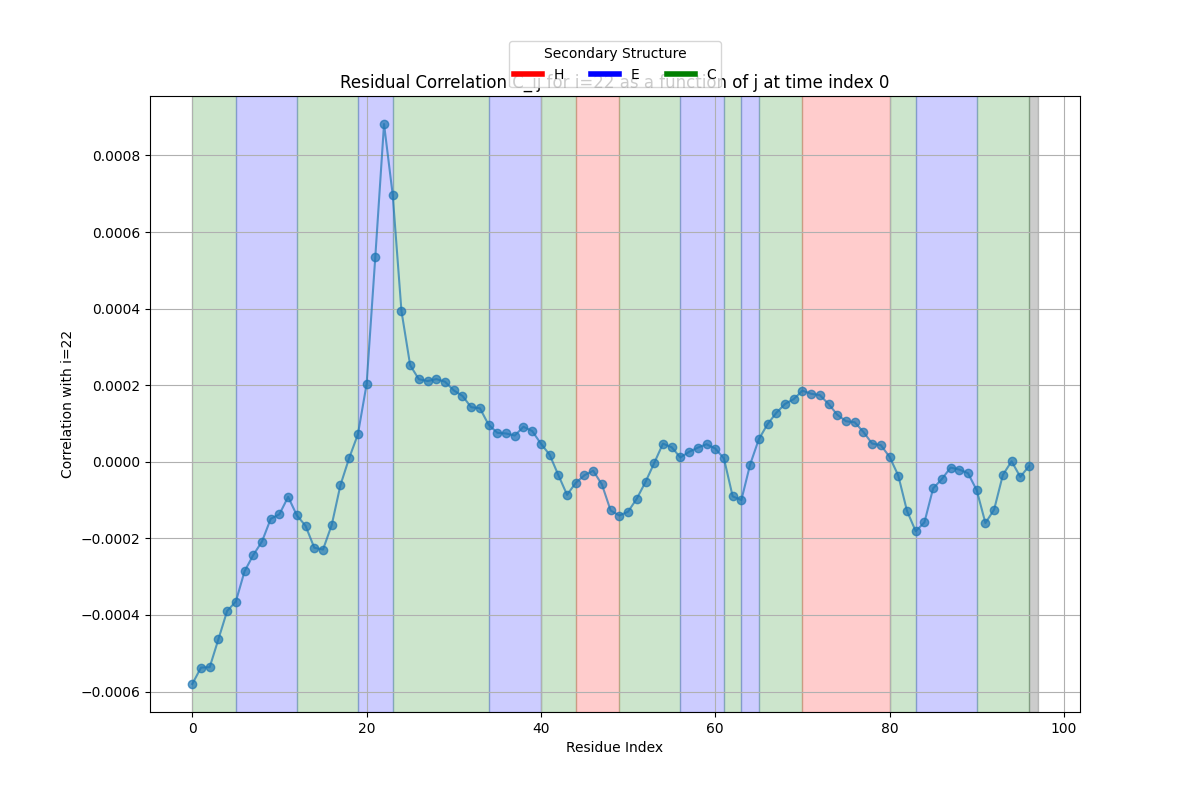
\includegraphics[width=0.5\textwidth]{images/2m0zResidual Correlation C_ij for i=22 as a function of j at time index 0.png}
    \caption{Correlazione}
\end{figure}
\begin{figure}[H]
    \centering
    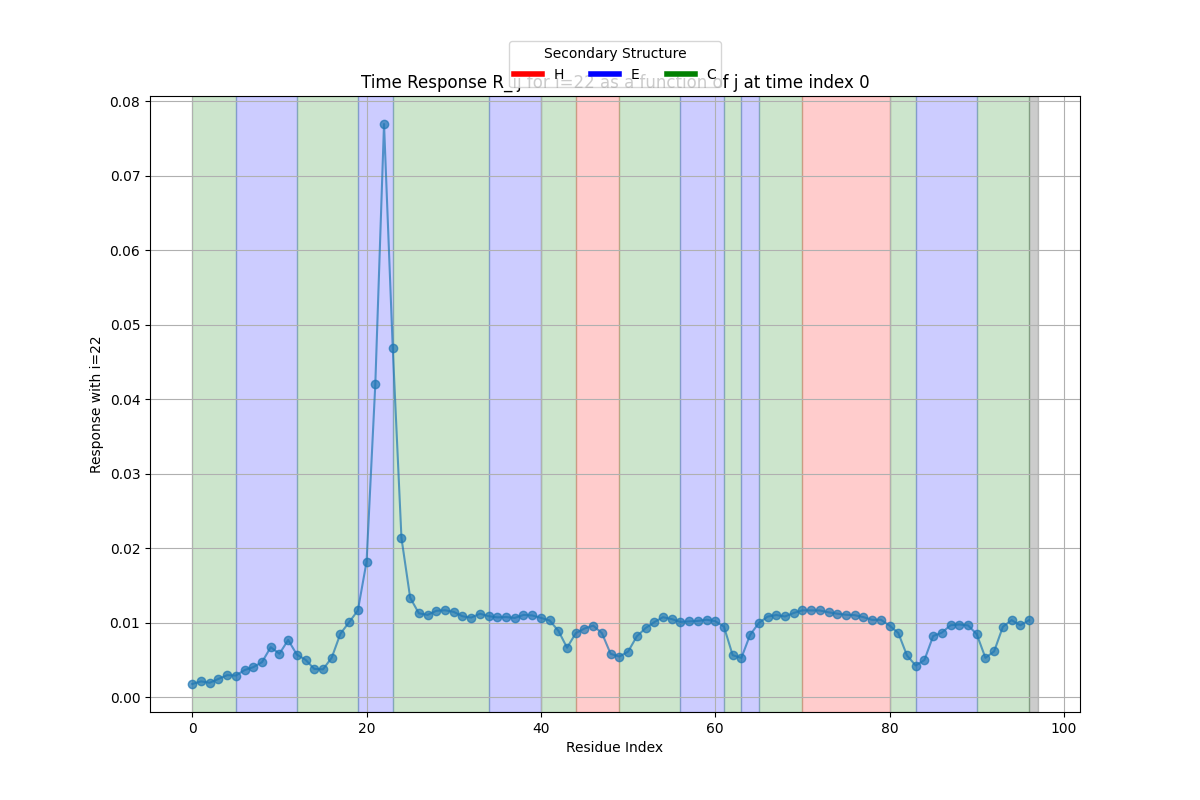
\includegraphics[width=0.5\textwidth]{"images/2m0zTime Response R_ij for i=22 as a function of j at time index 0.png"}
    \caption{Risposta}
\end{figure}

\begin{figure}[H]
    \centering
    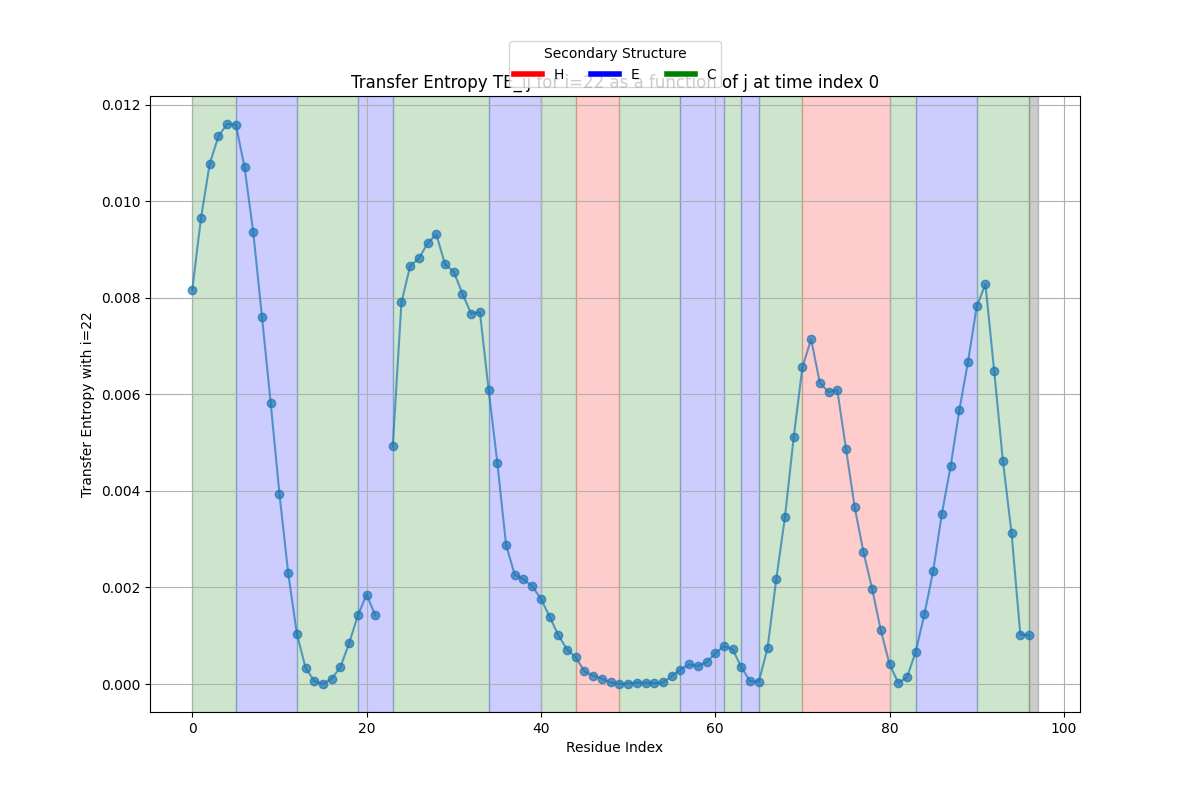
\includegraphics[width=0.5\textwidth]{"images/2m0zTransfer Entropy TE_ij for i=22 as a function of j at time index 0.png"}
    \caption{Transfer Entropy}
\end{figure}
\begin{figure}[H]
    \centering
    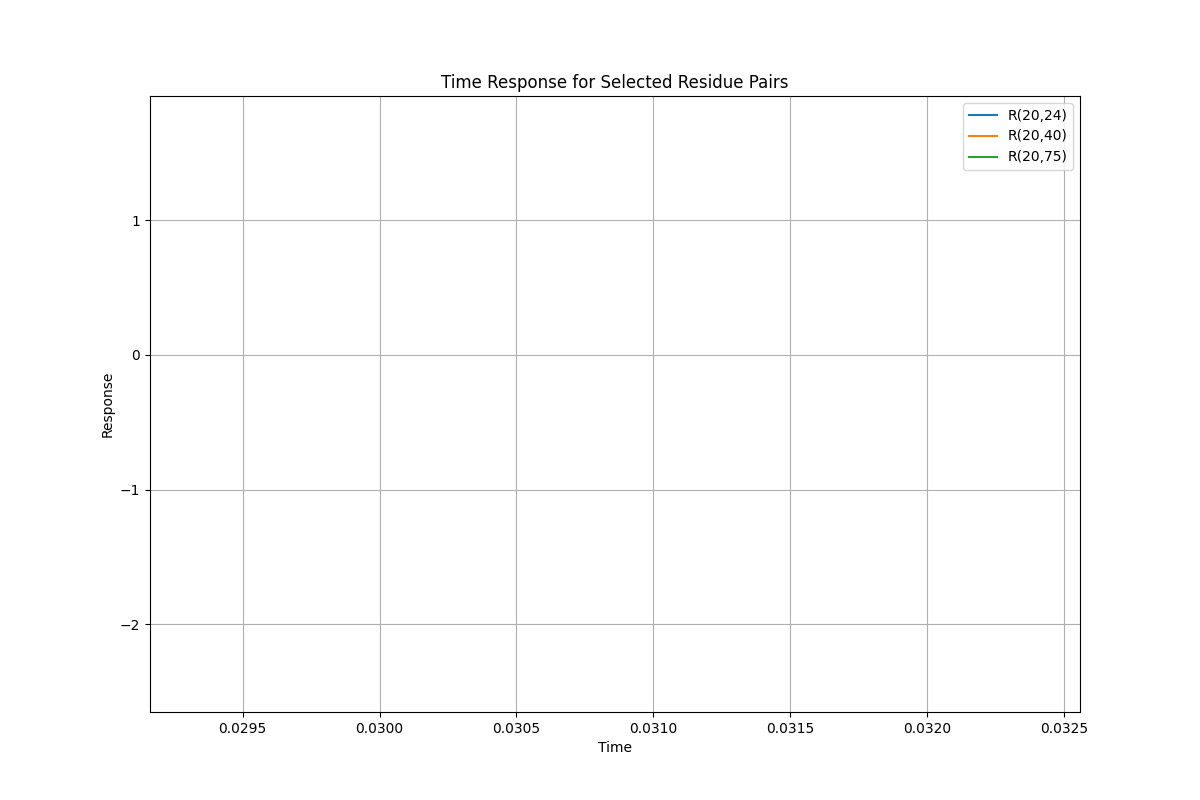
\includegraphics[width=0.5\textwidth]{"images/2m0zMultiple_time_resposne.png"}
    \caption{Multiple time response}
\end{figure}

\begin{figure}[H]
    \centering
    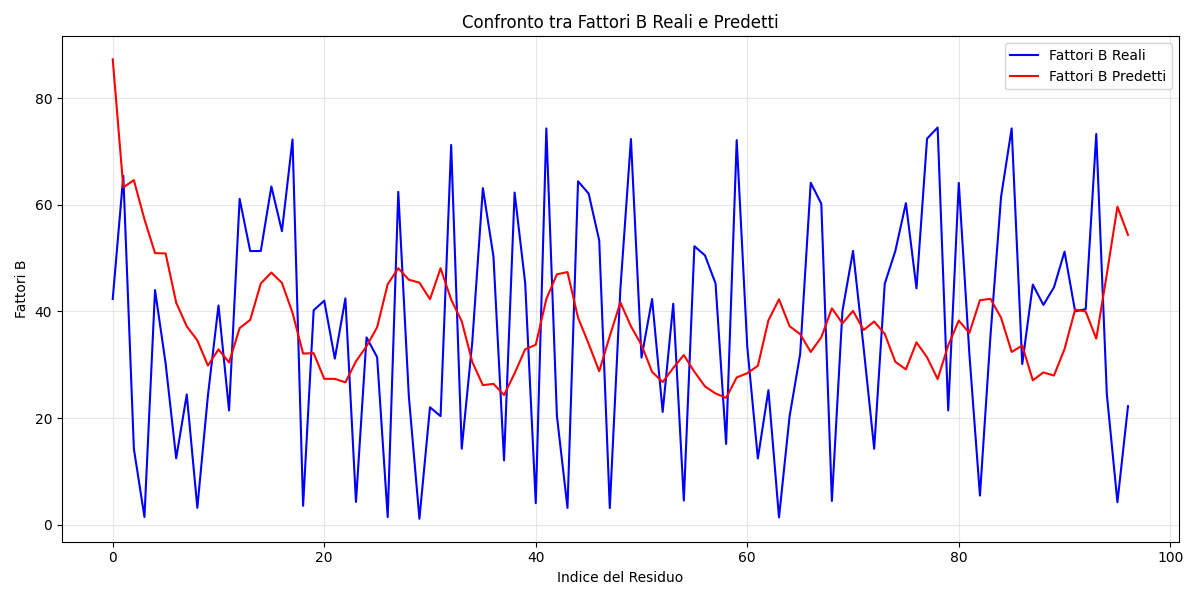
\includegraphics[width=0.5\textwidth]{"images/2m0zConfronto tra Fattori B Reali e Predetti.png"}
    \caption{B factors}
\end{figure}
\begin{figure}[H]
    \centering
    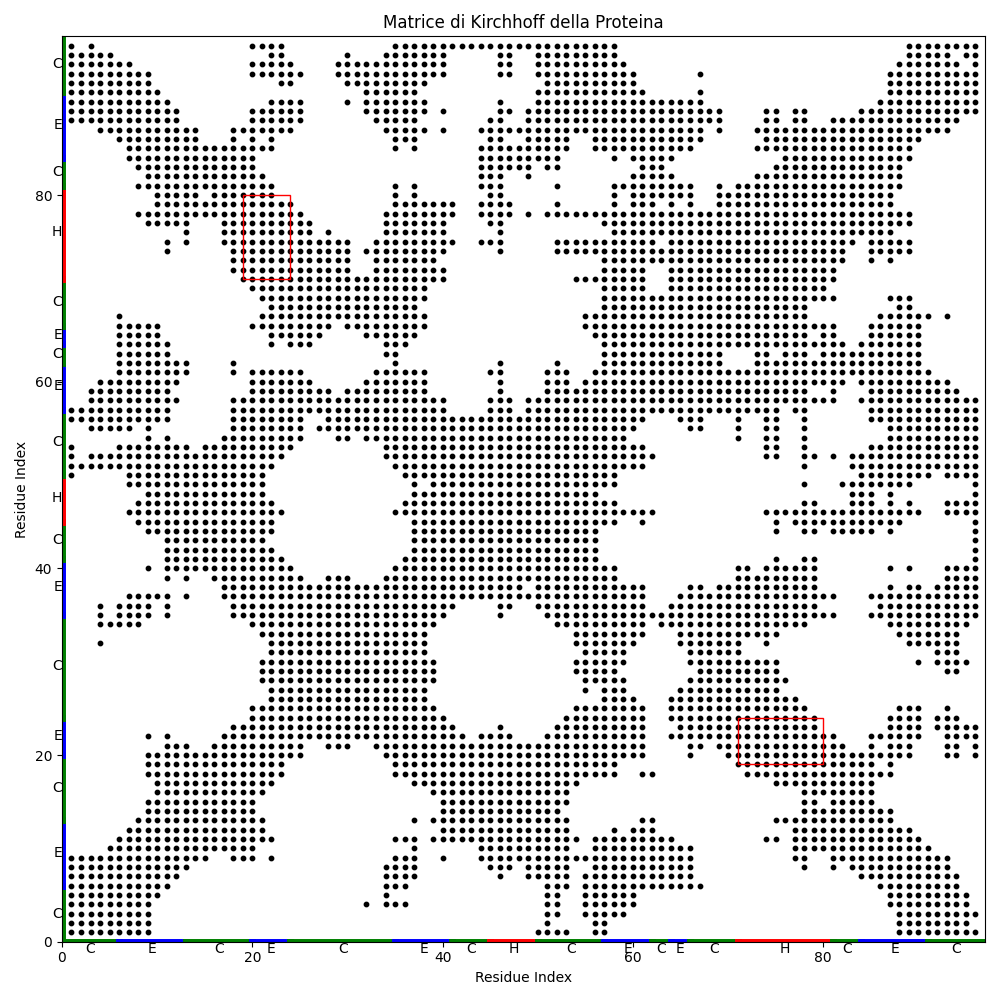
\includegraphics[width=0.5\textwidth]{"images/2m0z_Matrice di Kirchhoff della Proteina.png"}
    \caption{Kirchhoff}
\end{figure}
\begin{figure}[H]
    \centering
    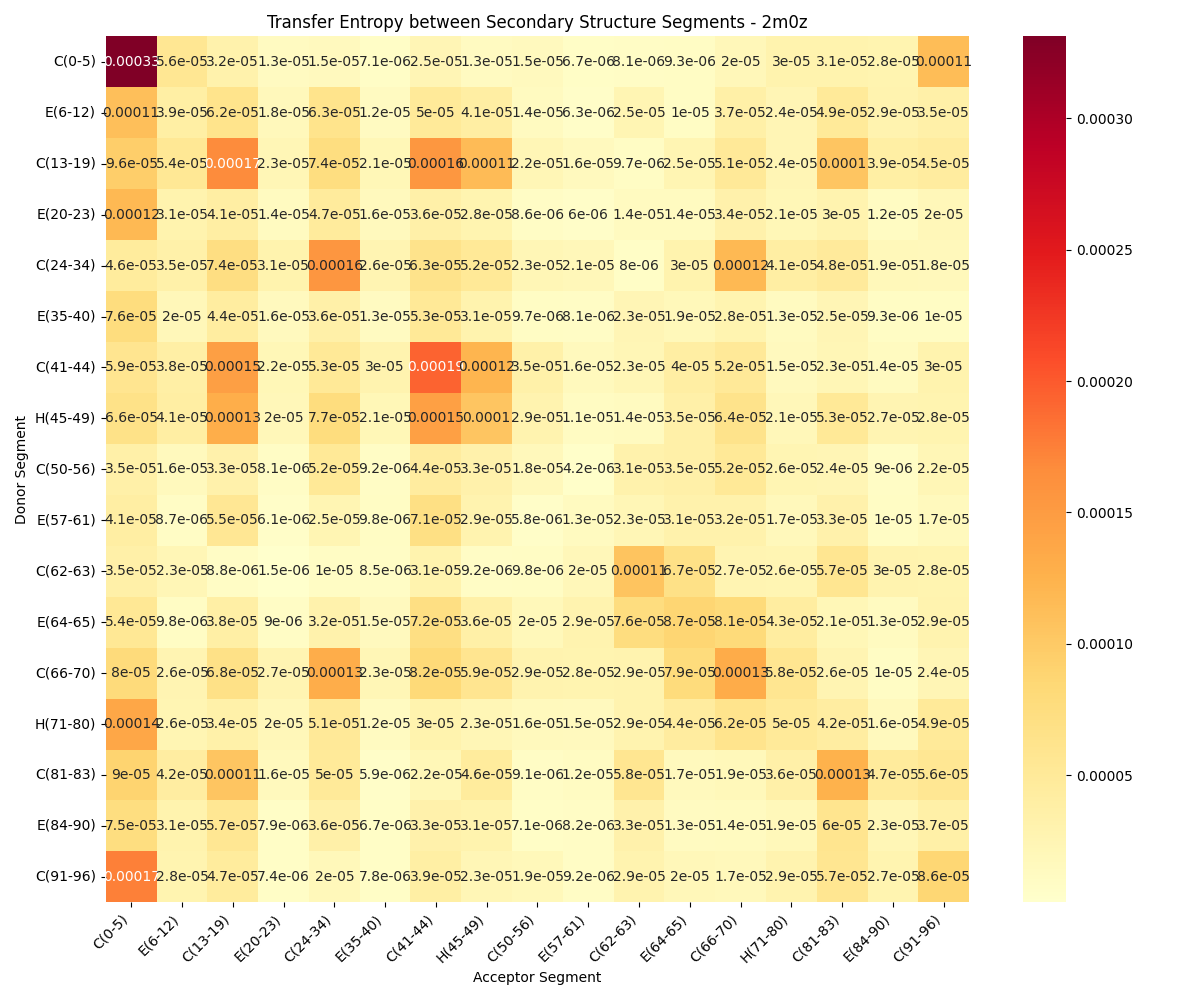
\includegraphics[width=0.5\textwidth]{"images/2m0zanalyze_secondary_structure_transfer_entropy.png"}
    \caption{Secodnaria Structure}
\end{figure}
\section{2M10}
\begin{figure}[H]
    \centering                            
    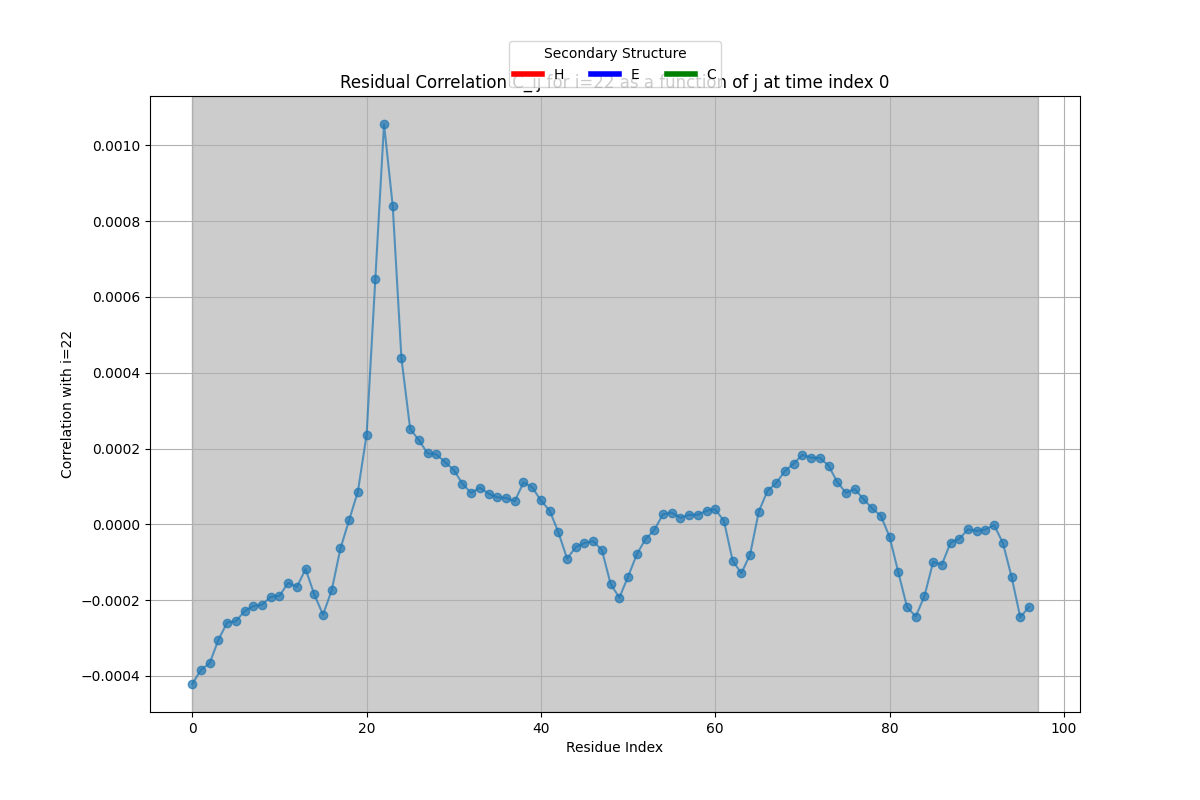
\includegraphics[width=0.5\textwidth]{"images/2m10Residual Correlation C_ij for i=22 as a function of j at time index 0.png"}
    \caption{Correlazione}
\end{figure}
\begin{figure}[H]
    \centering
    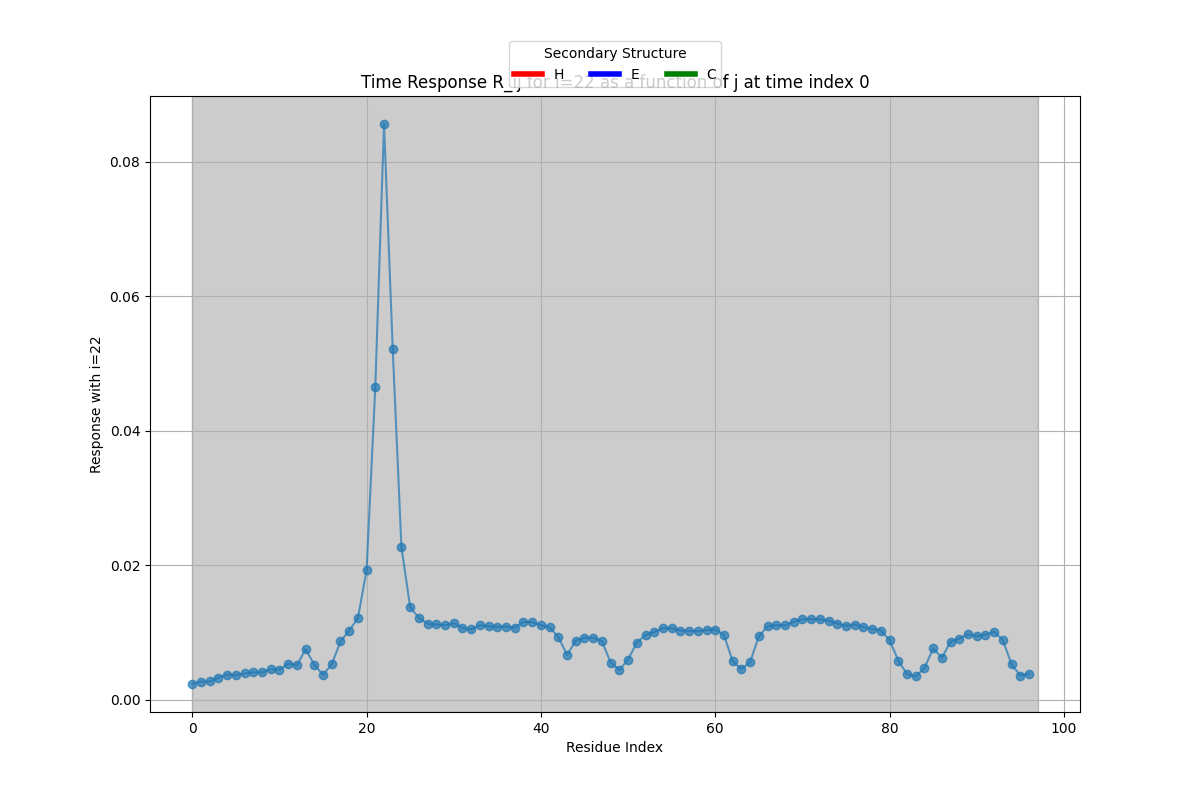
\includegraphics[width=0.5\textwidth]{"images/2m10Time Response R_ij for i=22 as a function of j at time index 0.png"}
    \caption{Risposta}
\end{figure}

\begin{figure}[H]
    \centering
    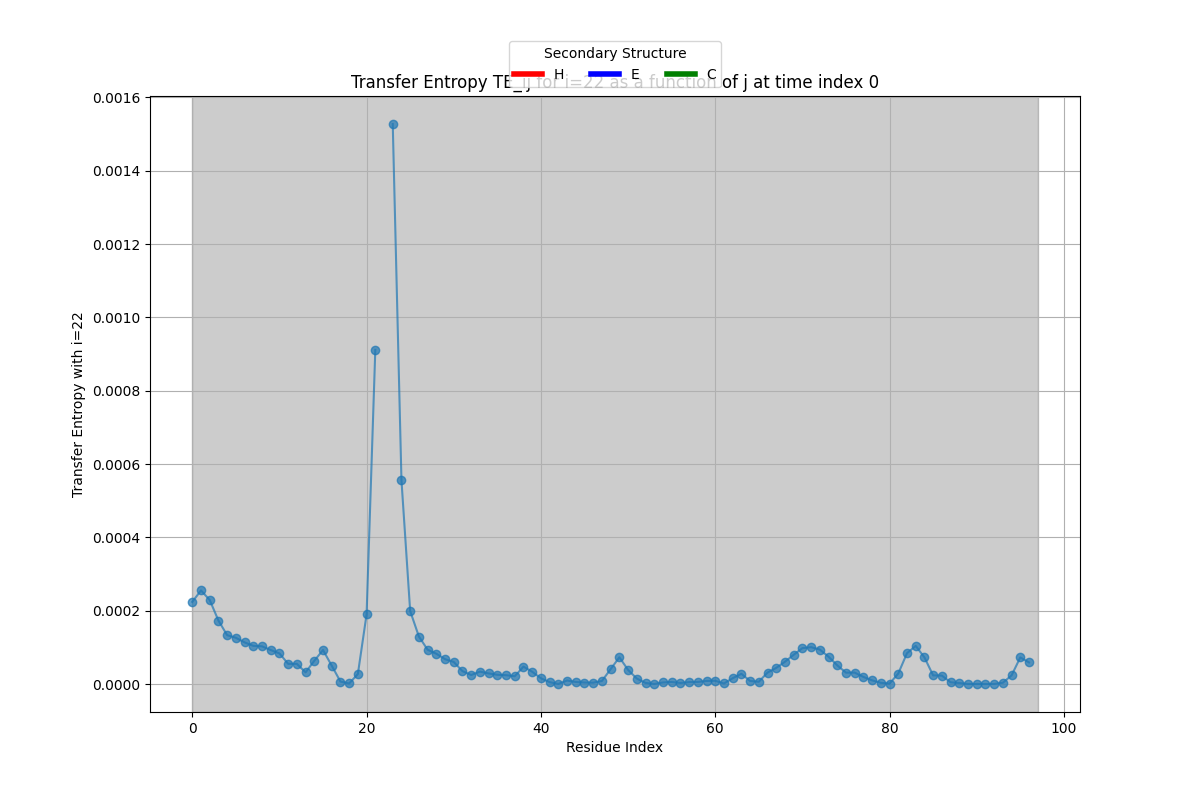
\includegraphics[width=0.5\textwidth]{"images/2m10Transfer Entropy TE_ij for i=22 as a function of j at time index 0.png"}
    \caption{Transfer Entropy}
\end{figure}
\begin{figure}[H]
    \centering
    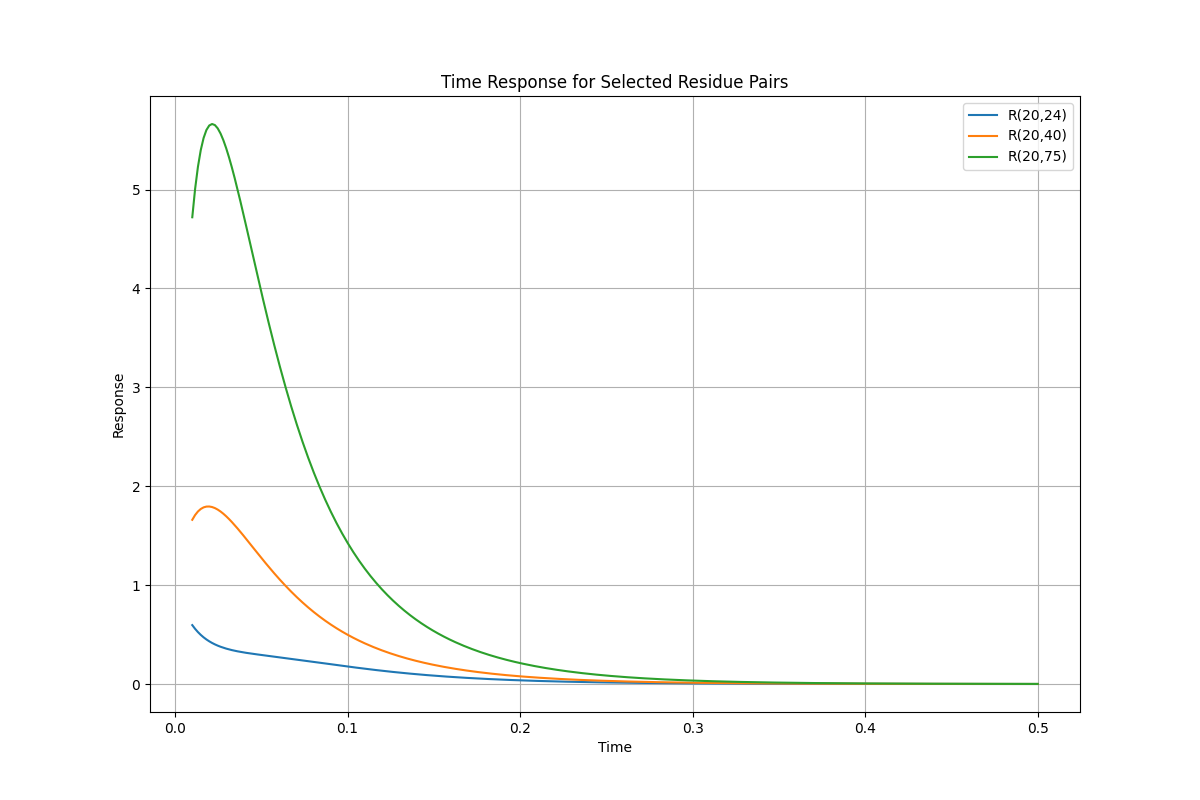
\includegraphics[width=0.5\textwidth]{"images/2m10Multiple_time_resposne.png"}
    \caption{Multiple time response}
\end{figure}

\begin{figure}[H]
    \centering
    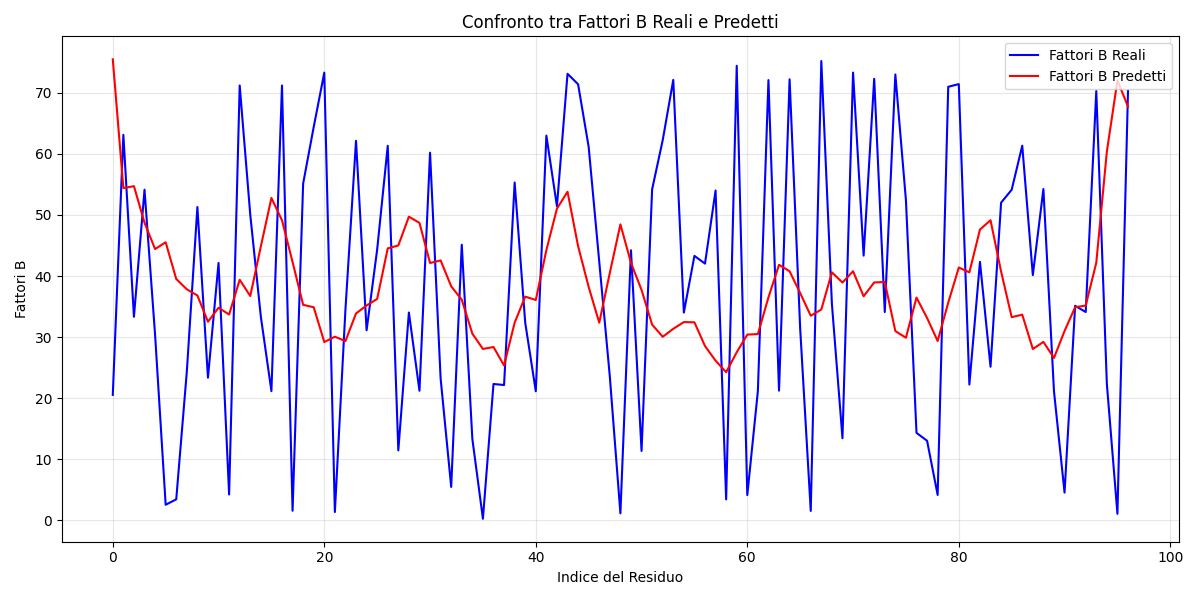
\includegraphics[width=0.5\textwidth]{"images/2m10Confronto tra Fattori B Reali e Predetti.png"}
    \caption{B factors}
\end{figure}
\begin{figure}[H]
    \centering
    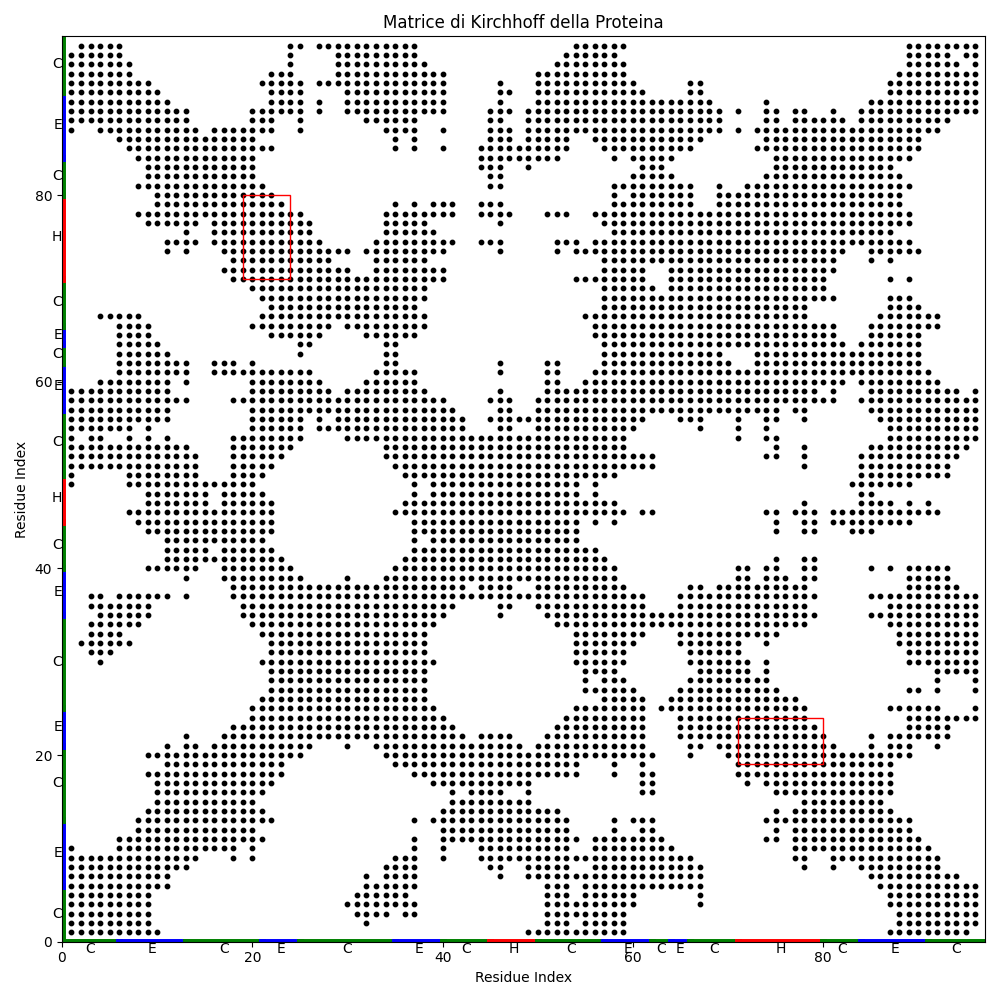
\includegraphics[width=0.5\textwidth]{"images/2m10_Matrice di Kirchhoff della Proteina.png"}
    \caption{Kirchhoff}
\end{figure}
\begin{figure}[H]
    \centering
    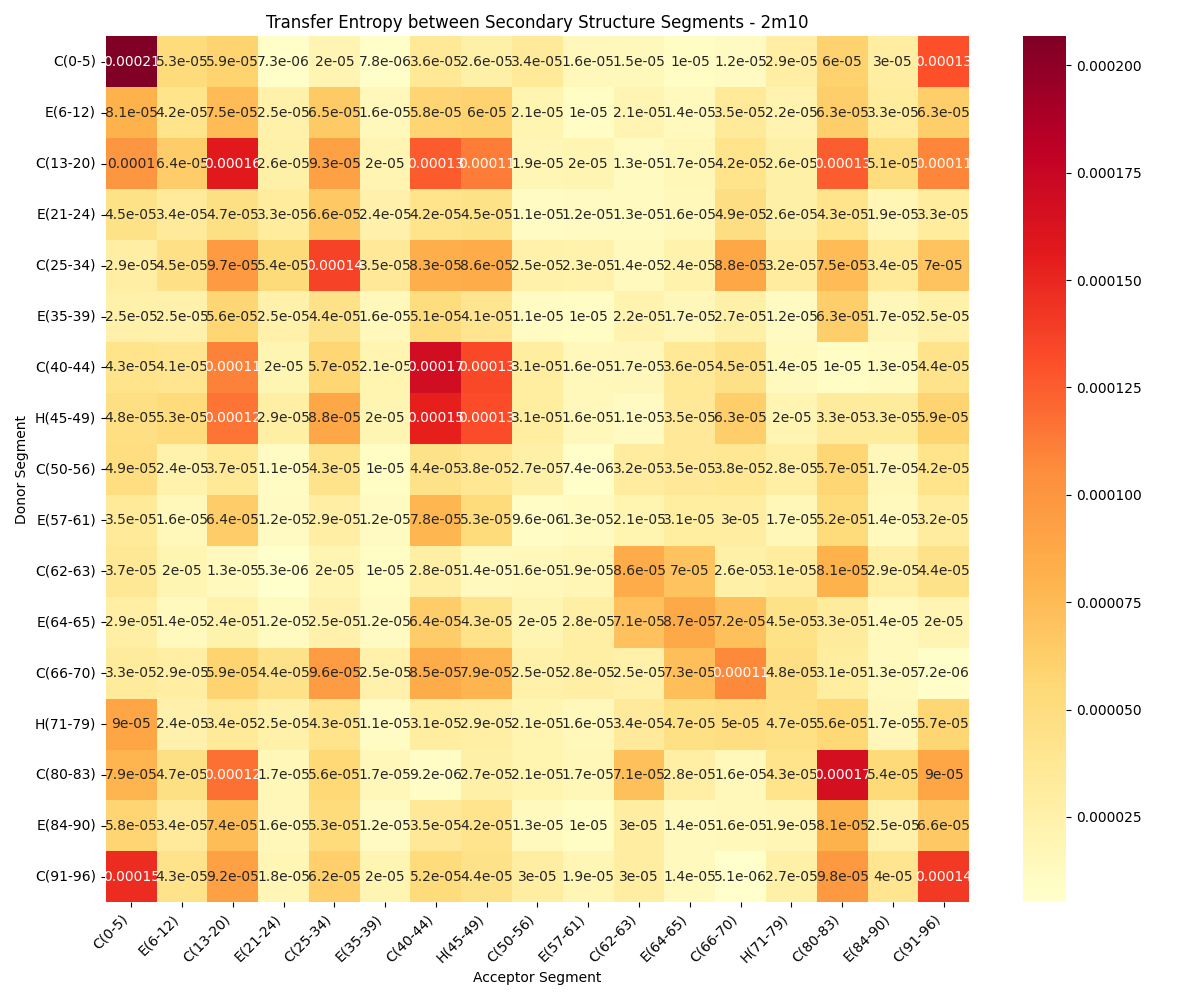
\includegraphics[width=0.5\textwidth]{"images/2m10analyze_secondary_structure_transfer_entropy.png"}
    \caption{Transfer struttura Secondaria}
\end{figure}
\section{3LNX}
\begin{figure}[H]
    \centering
    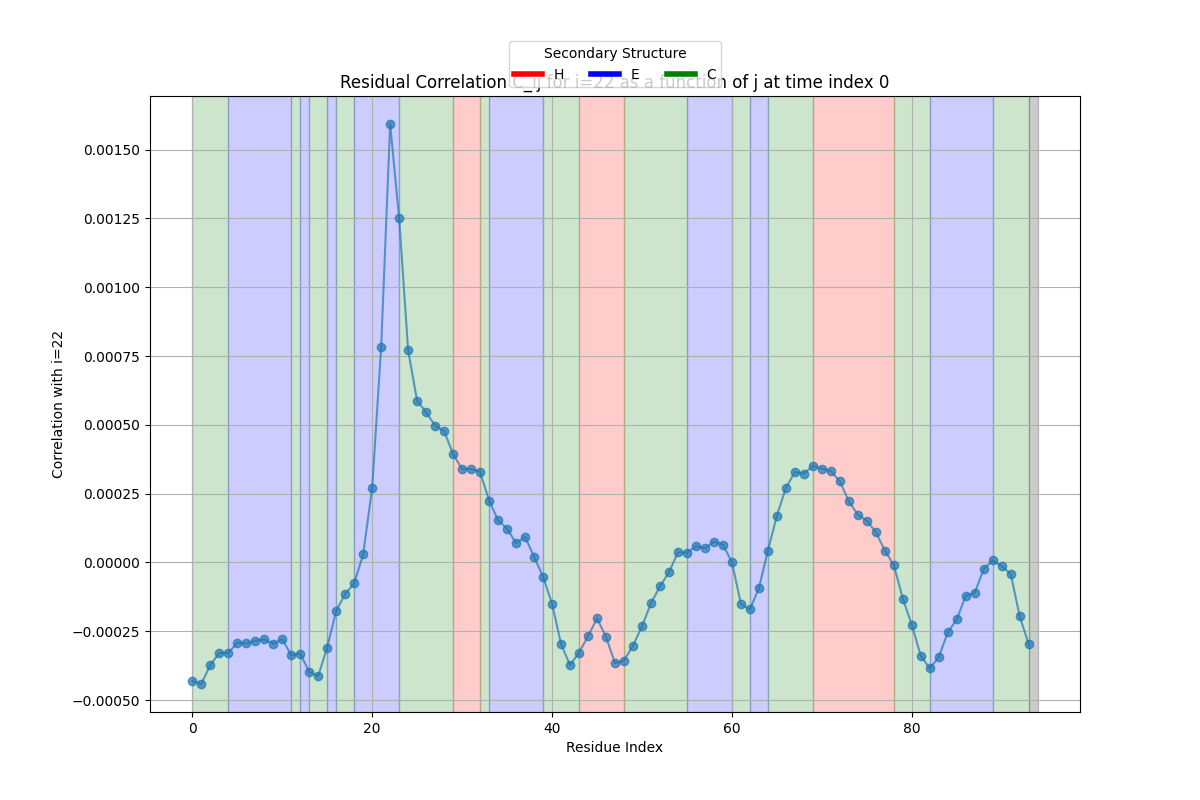
\includegraphics[width=0.5\textwidth]{"images/3LNXResidual Correlation C_ij for i=22 as a function of j at time index 0.png"}
    \caption{Correlazione}
\end{figure}
\begin{figure}[H]
    \centering
    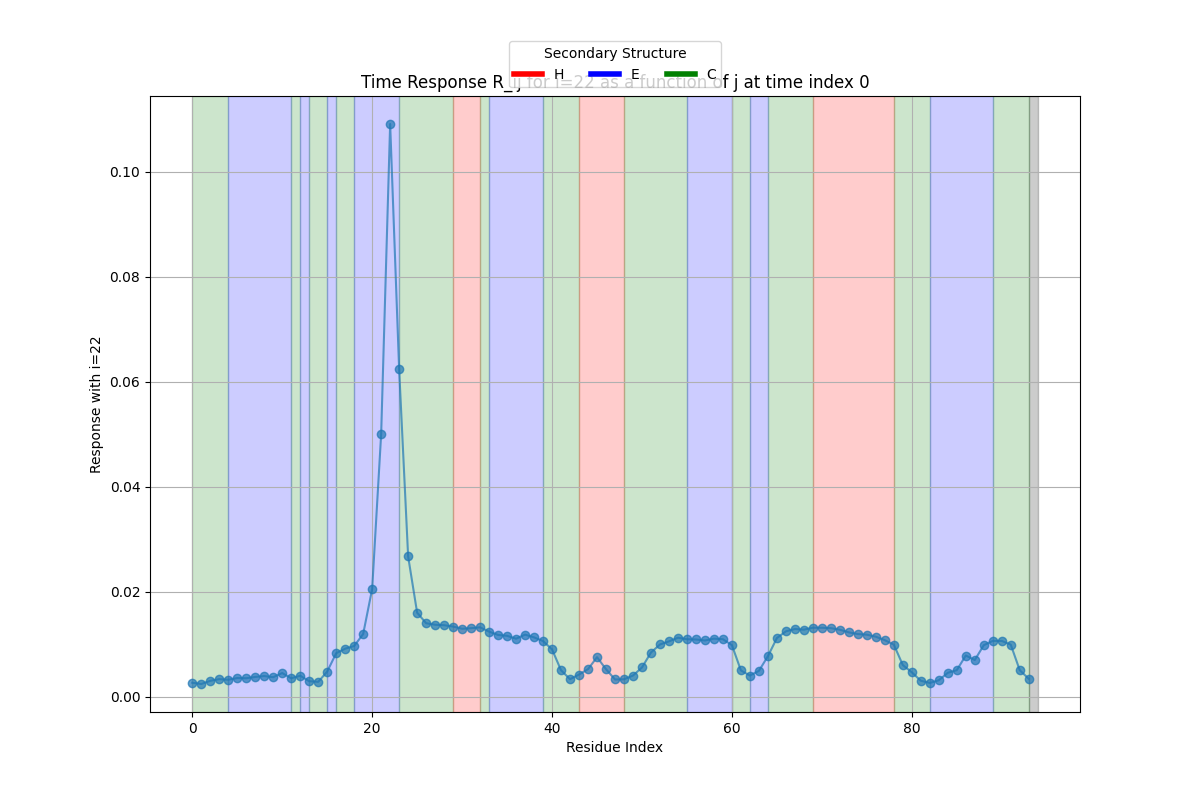
\includegraphics[width=0.5\textwidth]{"images/3LNXTime Response R_ij for i=22 as a function of j at time index 0.png"}
    \caption{Risposta}
\end{figure}

\begin{figure}[H]
    \centering
    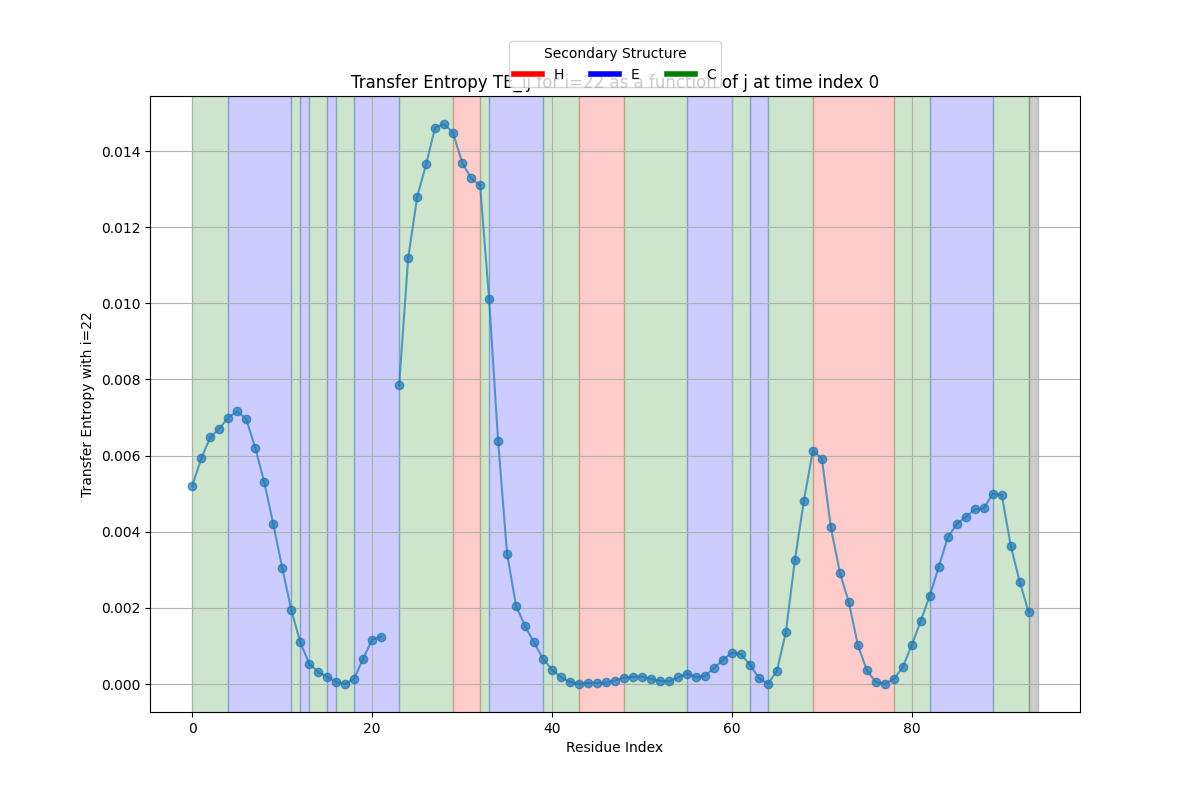
\includegraphics[width=0.5\textwidth]{"images/3LNXTransfer Entropy TE_ij for i=22 as a function of j at time index 0.png"}
    \caption{Transfer Entropy}
\end{figure}
\begin{figure}[H]
    \centering
    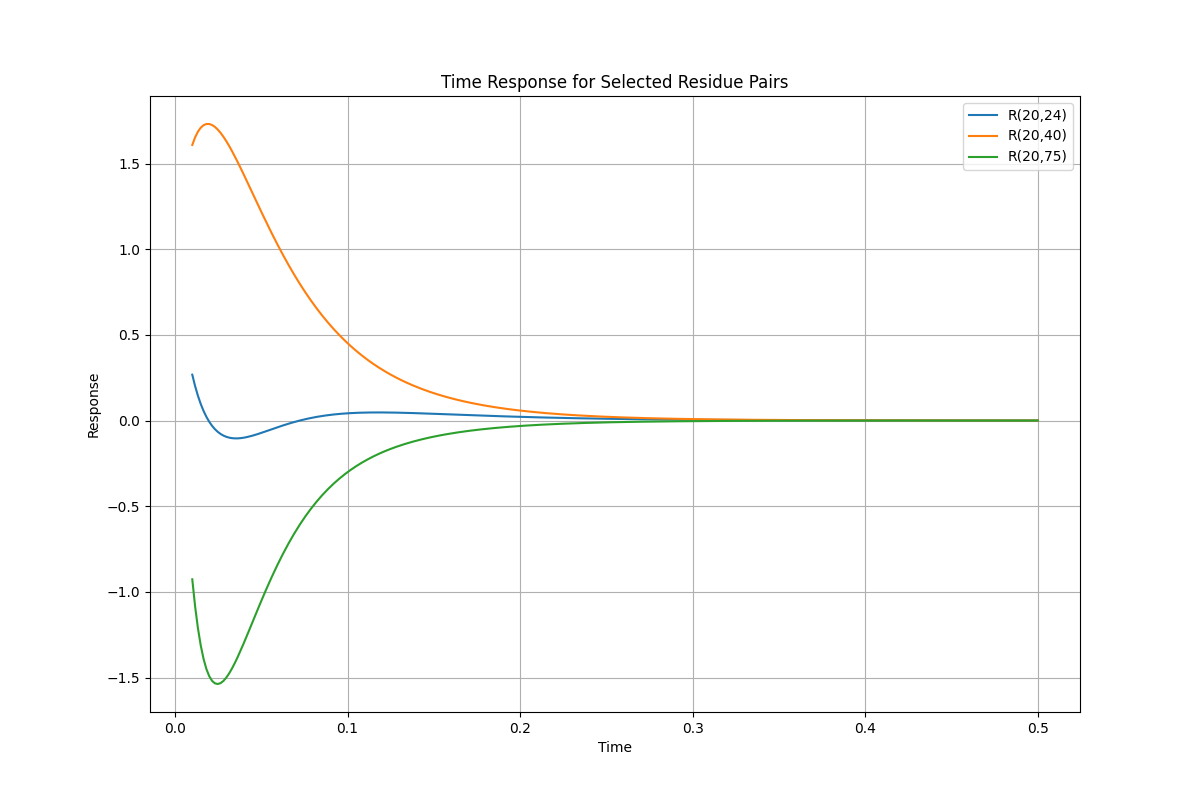
\includegraphics[width=0.5\textwidth]{"images/3LNXMultiple_time_resposne.png"}
    \caption{Multiple time response}
\end{figure}

\begin{figure}[H]
    \centering
    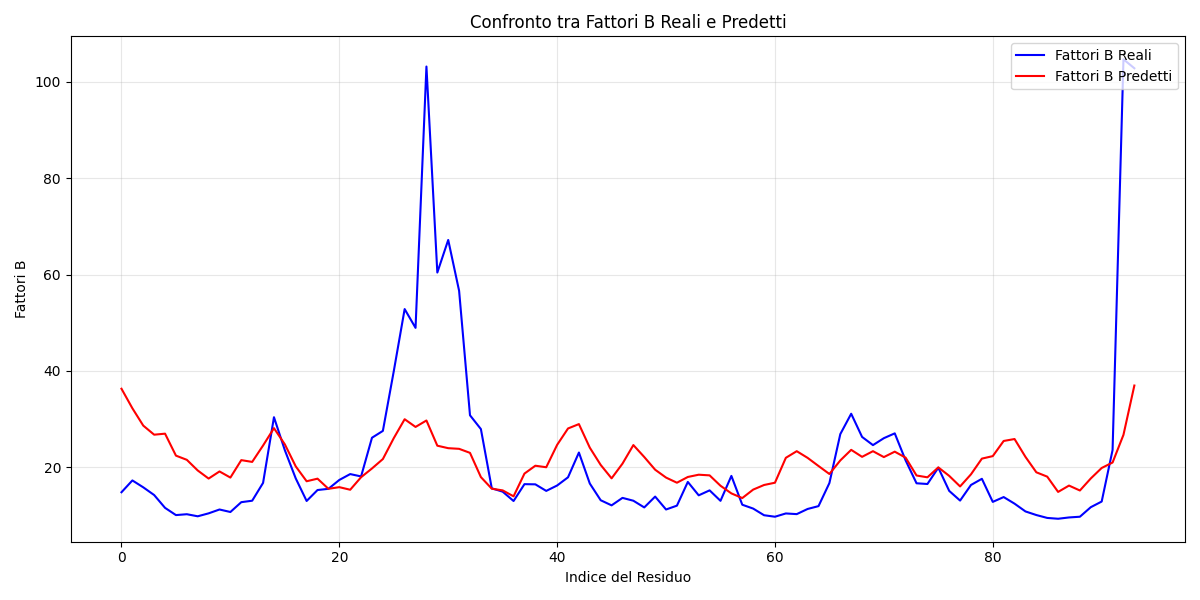
\includegraphics[width=0.5\textwidth]{"images/3LNXConfronto tra Fattori B Reali e Predetti.png"}
    \caption{B factors}
\end{figure}
\begin{figure}[H]
    \centering
    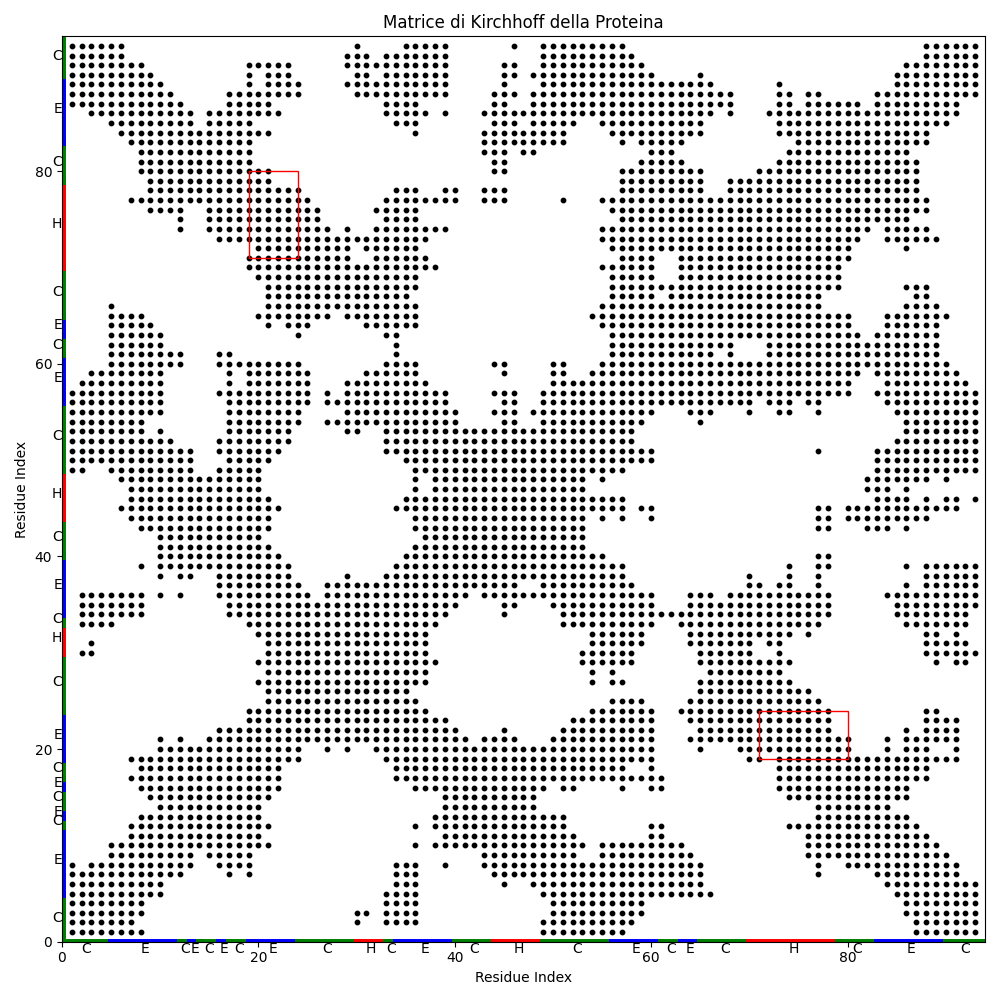
\includegraphics[width=0.5\textwidth]{"images/3LNX_Matrice di Kirchhoff della Proteina.png"}
    \caption{Kirchhoff}
\end{figure}
\begin{figure}[H]
    \centering
    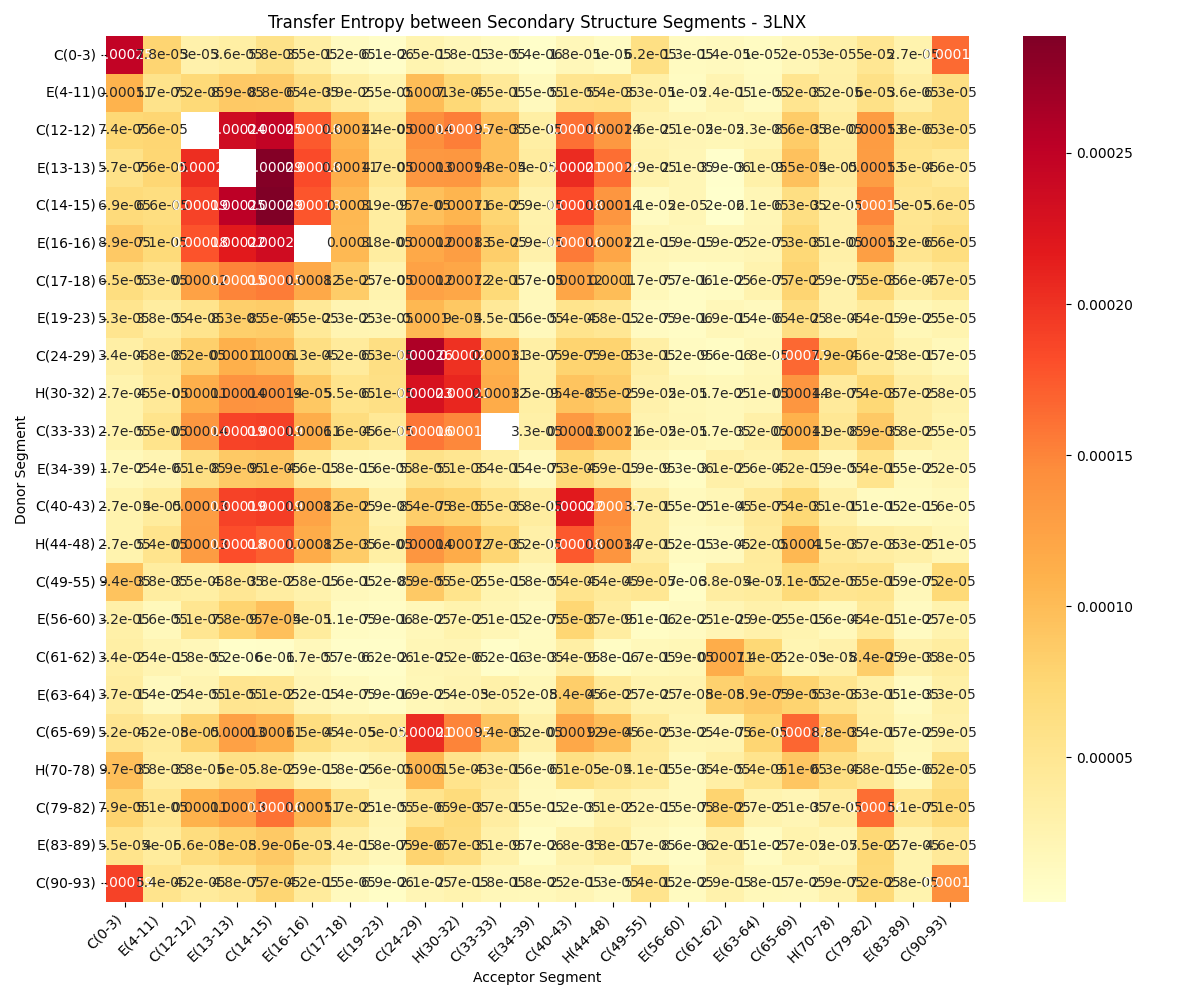
\includegraphics[width=0.5\textwidth]{"images/3LNXanalyze_secondary_structure_transfer_entropy.png"}
    \caption{Secondaria}
\end{figure}
\section{3LNY}
\begin{figure}[H]
    \centering
    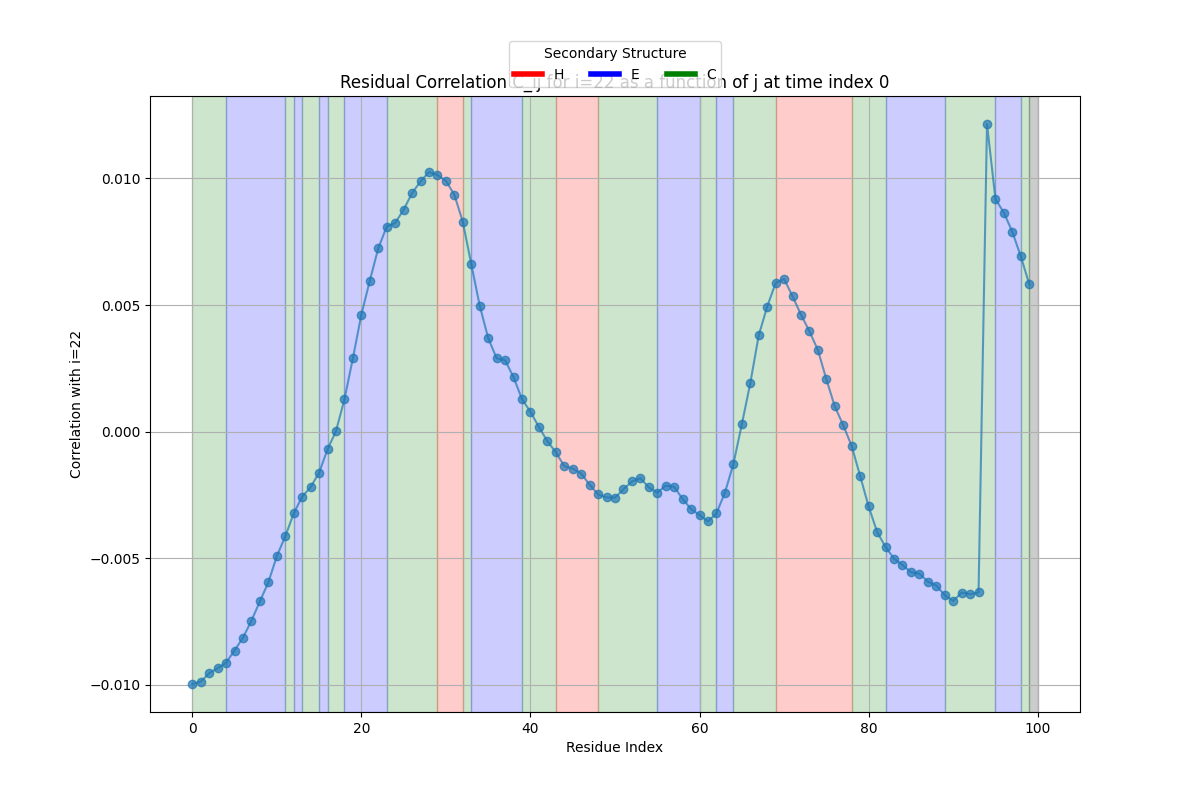
\includegraphics[width=0.5\textwidth]{"images/3LNYResidual Correlation C_ij for i=22 as a function of j at time index 0.png"}
    \caption{Correlazione}
\end{figure}
\begin{figure}[H]
    \centering
    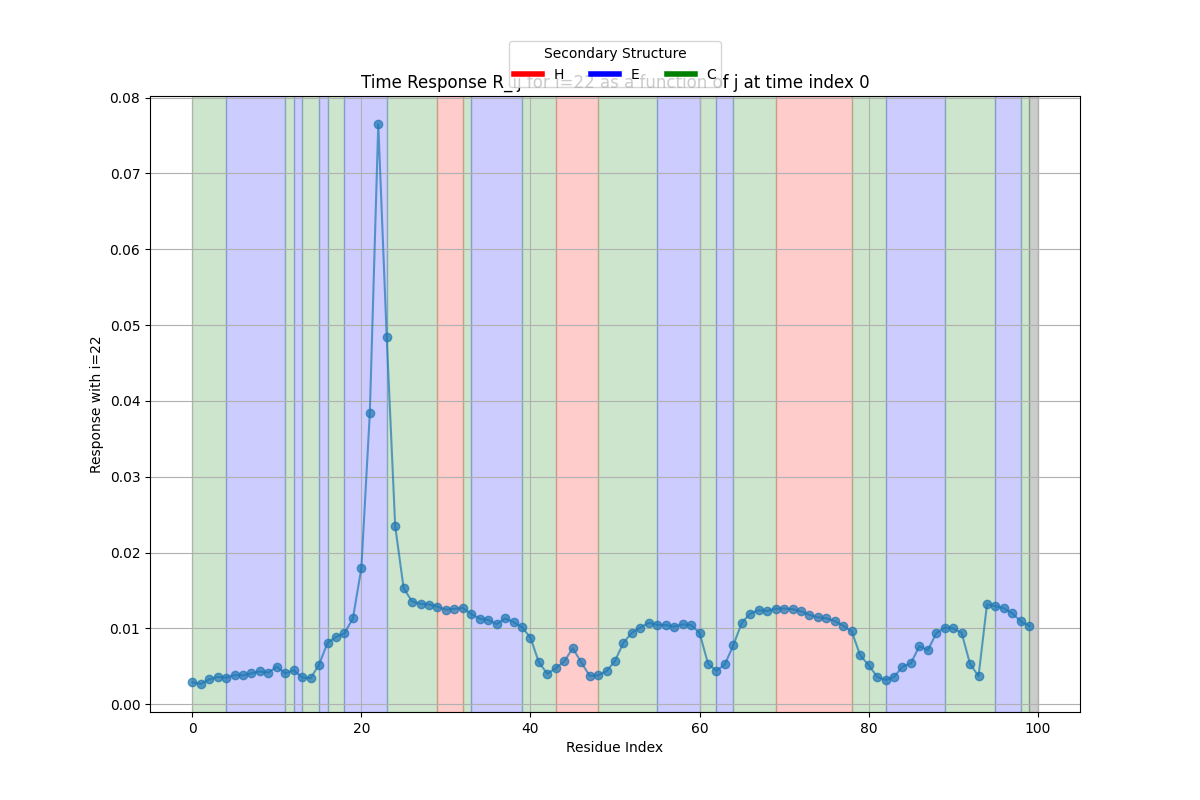
\includegraphics[width=0.5\textwidth]{"images/3LNYTime Response R_ij for i=22 as a function of j at time index 0.png"}
    \caption{Risposta}
\end{figure}

\begin{figure}[H]
    \centering
    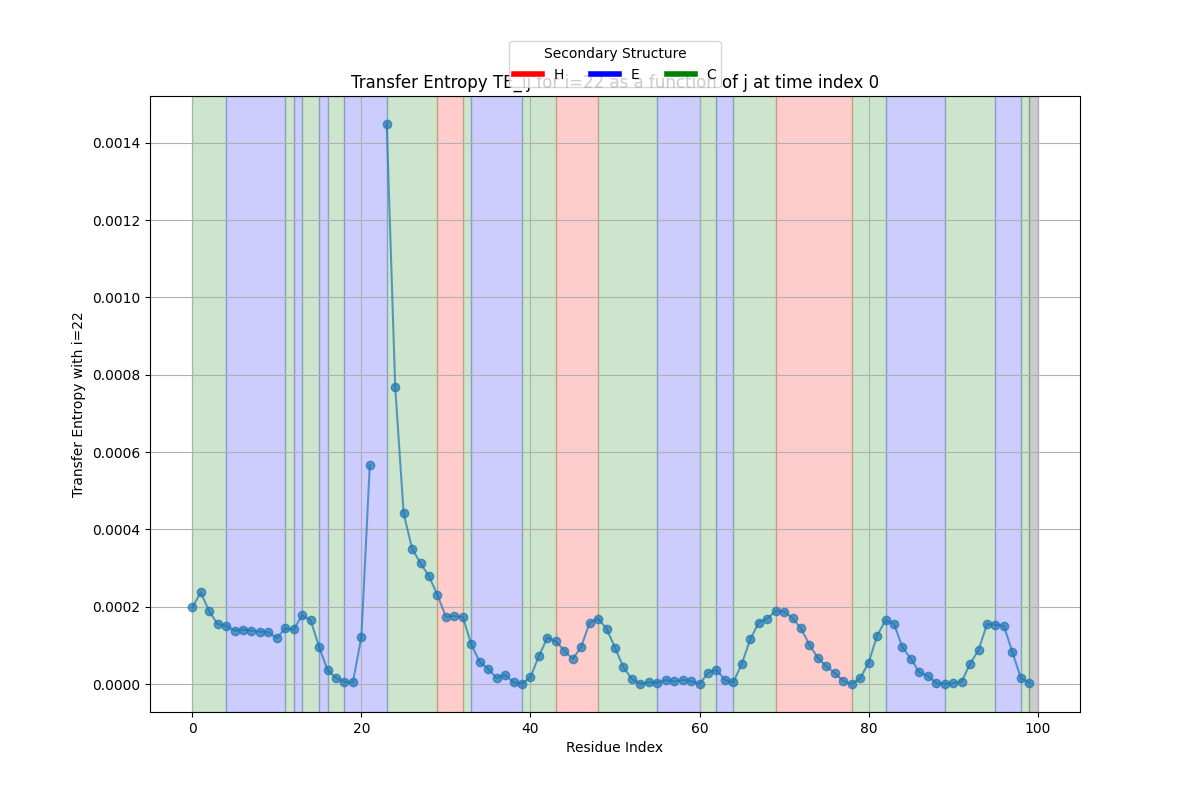
\includegraphics[width=0.5\textwidth]{"images/3LNYTransfer Entropy TE_ij for i=22 as a function of j at time index 0.png"}
    \caption{Transfer Entropy}
\end{figure}


\begin{figure}[H]
    \centering
    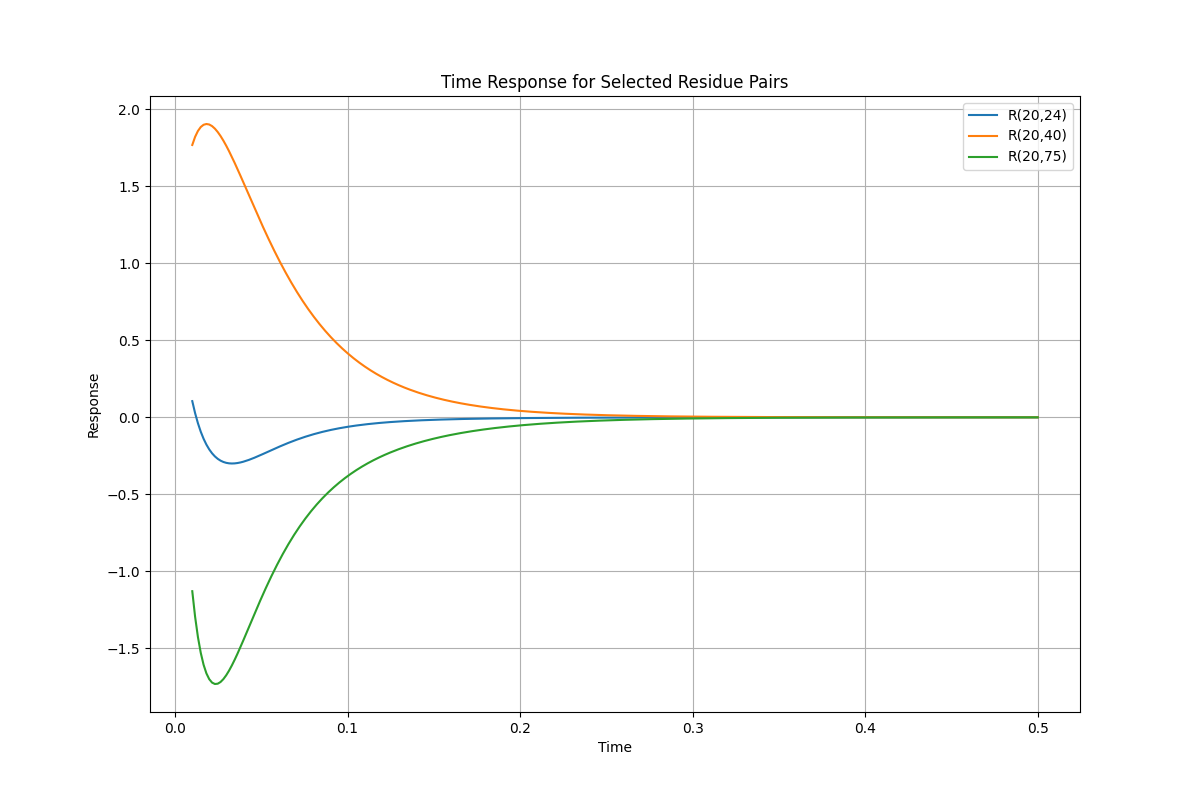
\includegraphics[width=0.5\textwidth]{"images/3LNYMultiple_time_resposne.png"}
    \caption{Multiple time response}
\end{figure}

\begin{figure}[H]
    \centering
    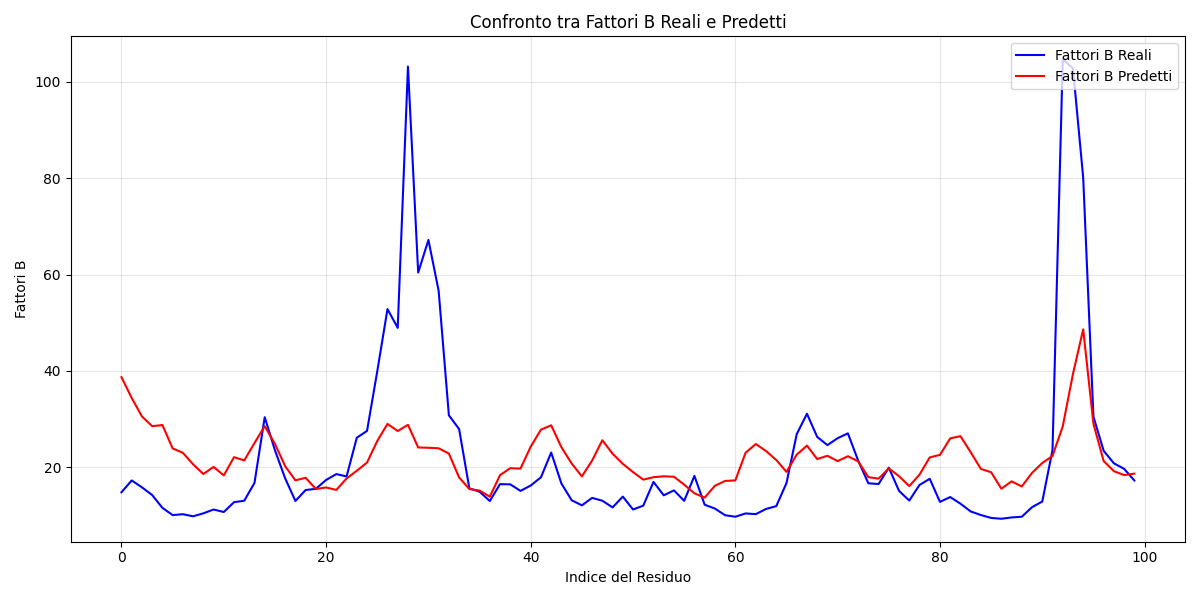
\includegraphics[width=0.5\textwidth]{"images/3LNYConfronto tra Fattori B Reali e Predetti.png"}
    \caption{B factors}
\end{figure}
\begin{figure}[H]
    \centering
    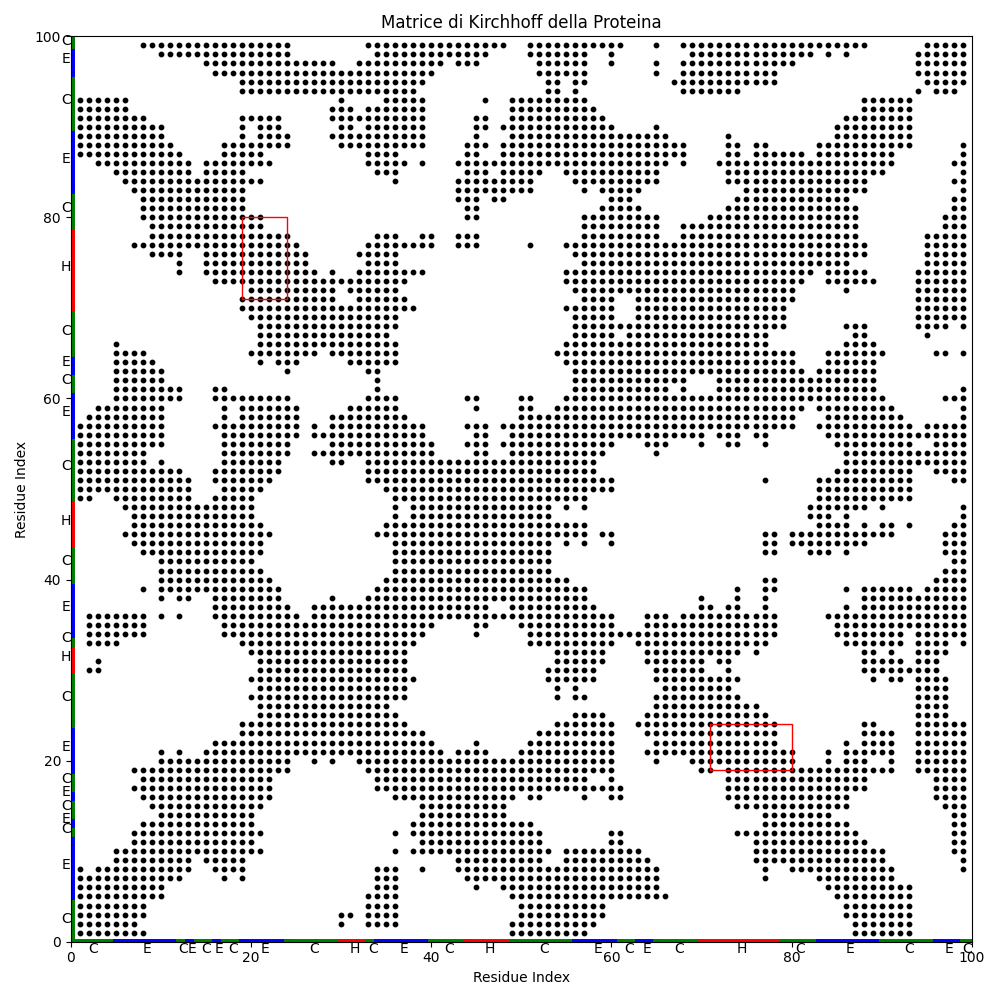
\includegraphics[width=0.5\textwidth]{"images/3LNY_Matrice di Kirchhoff della Proteina.png"}
    \caption{Kirchhoff}
\end{figure}
\begin{figure}[H]
    \centering
    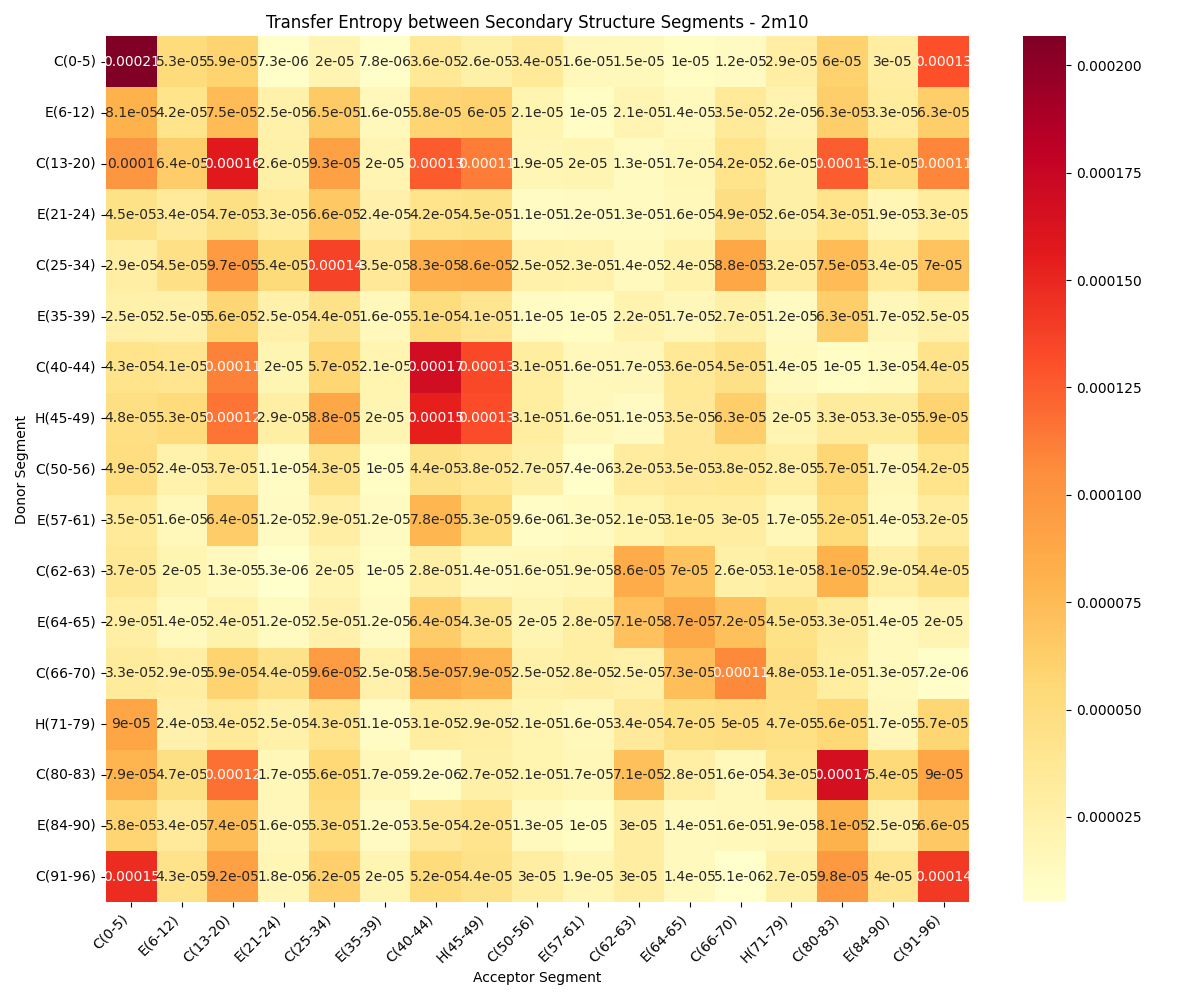
\includegraphics[width=0.5\textwidth]{"images/2m10analyze_secondary_structure_transfer_entropy.png"}
    \caption{Seocndaria}
\end{figure}
\section{Dinamica}
\begin{equation}
    \gamma \dot{x}_i = -g \sum_j K_{ij} x_j + \epsilon(t) (r_{21} - r_{76}) \delta_{i,21} - \epsilon(t) (r_{21} - r_{76}) \delta_{i,76} + \sqrt{2 \gamma k_B T} \xi_i(t)
    \end{equation}
Ora posso simulare il moto Time dependent di ogni atomo e vedere come si propagano le vibrazioni.
Gli autovalori sono smere le frequeze naturali del sistema.
\begin{figure}[H]
    \centering
    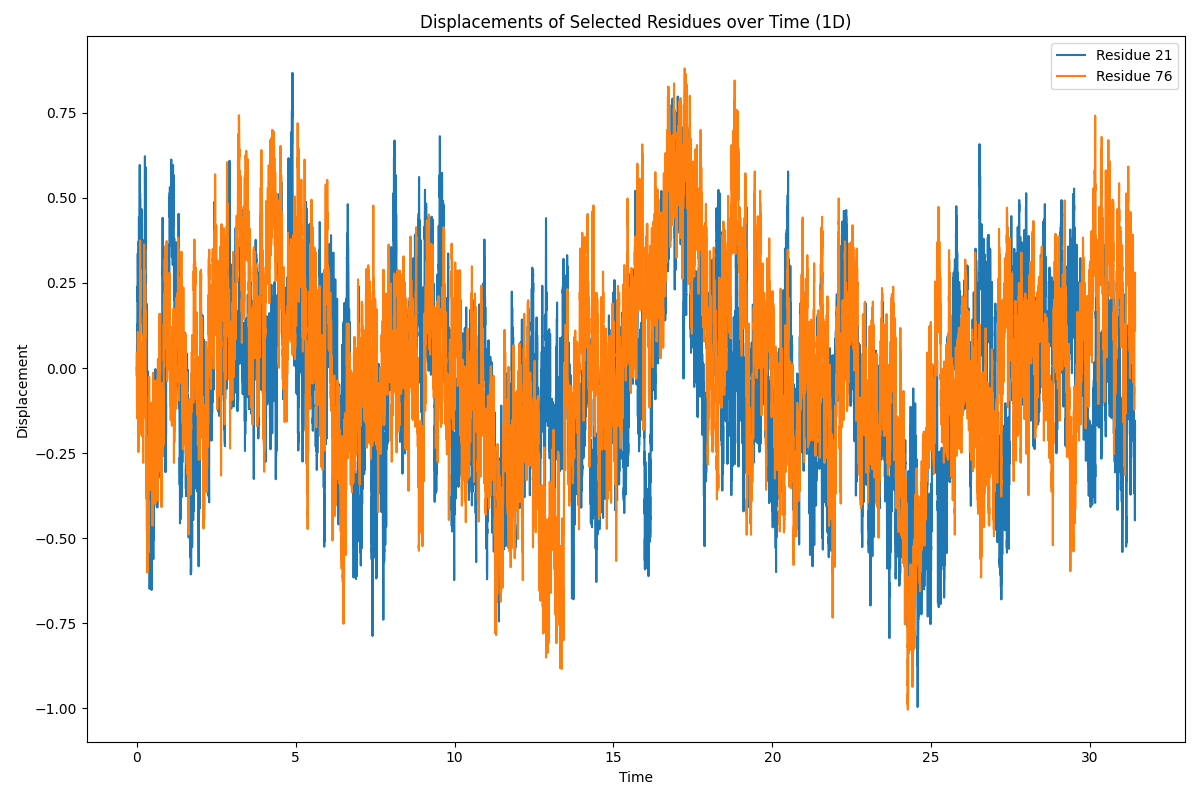
\includegraphics[width=0.5\textwidth]{"images/2m10_Processo_stocastico.png"}
    \caption{Seocndaria}
\end{figure}
\begin{figure}[H]
    \centering
    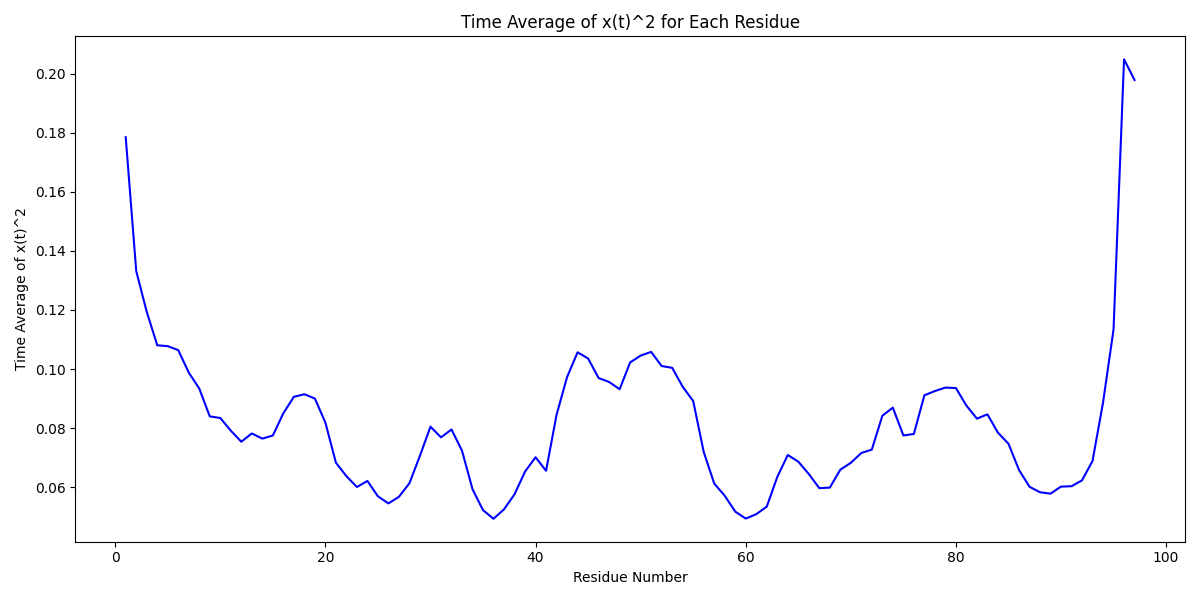
\includegraphics[width=0.5\textwidth]{"images/2m10_Stima beta factors.png"}
    \caption{Seocndaria}
\end{figure}
\section{Gradienete di temperature}
\begin{equation}
    \boldsymbol{\gamma}_i \dot{x}_i = -g \sum_j K_{ij} x_j  + \sqrt{2 \boldsymbol{\gamma}_i k_B \boldsymbol{T}_i} \xi_i(t)
    \end{equation}
Gamma e T sono diventati vettori.
Se la risolvi ottieni:
\begin{equation}
    \sum_{u} \exp\left( \sum_j K_{ij} u_j \right) \cdot \beta \cdot \beta^{\top} \cdot \exp\left( \sum_s K_{is} u_s \right)
    \end{equation}
Ora hai diversi modi di scegliere i valori di T:
\section{Troncamento Tmeperatura}
se sono sotto 5 legami allora ho temperatura bassa.
Se sono sopra allora ho temperatura piu' alta.
Posso prendere banalmente 2 valori 0,1 .
\begin{figure}[H]
    \centering
    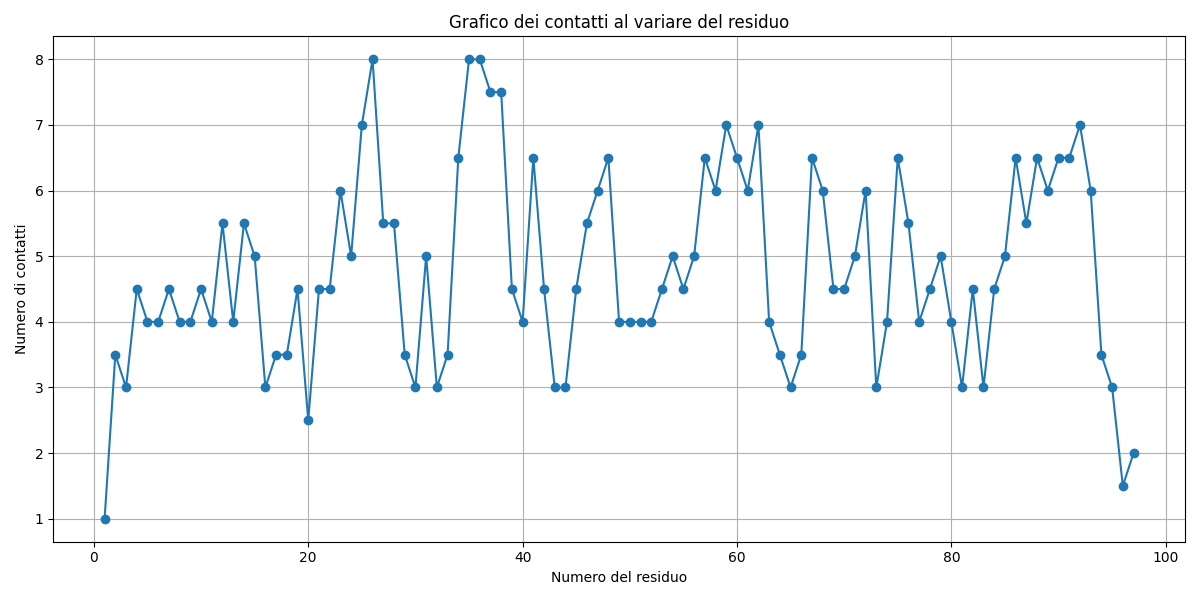
\includegraphics[width=0.5\textwidth]{"images/2m10_2_temperature_contact_cutoff.png"}
    \caption{ Temperatura Troncamento }
\end{figure}
\begin{figure}[H]
    \centering
    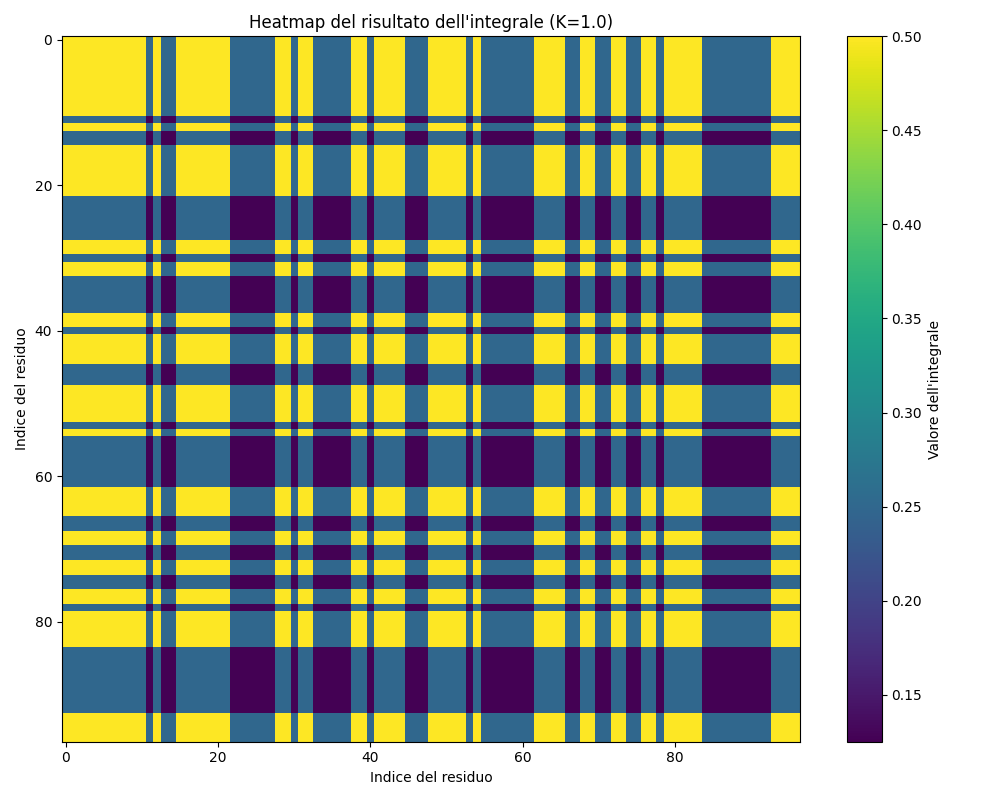
\includegraphics[width=0.5\textwidth]{"images/2m10_2_temperature_correlation_cutoff.png"}
    \caption{ Temperatura Troncamento  }
\end{figure}
\begin{figure}[H]
    \centering
    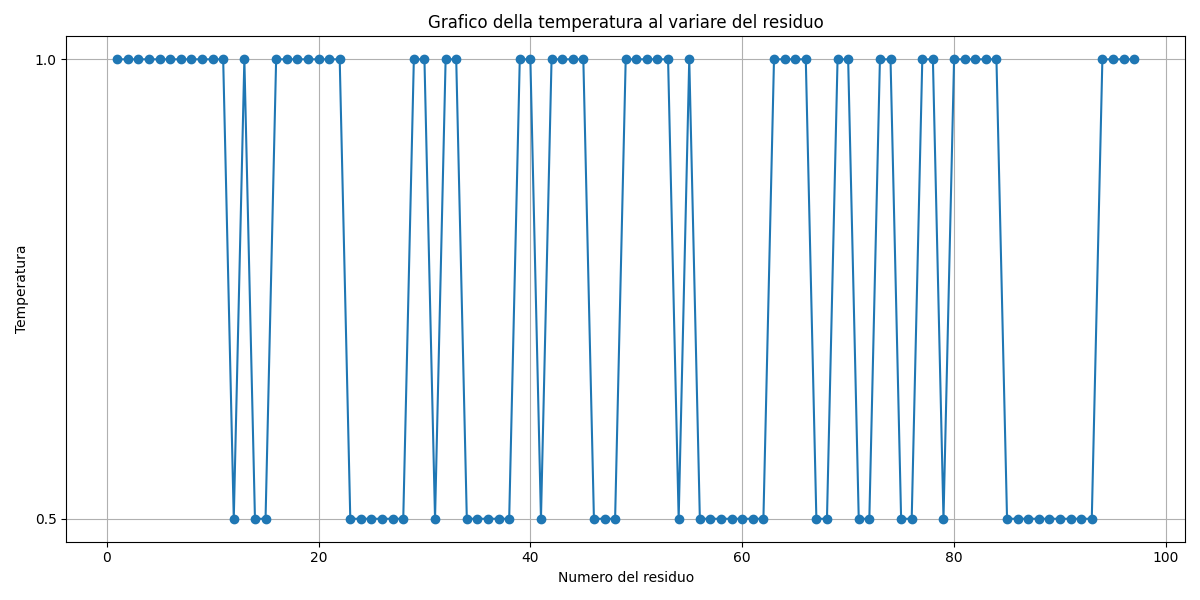
\includegraphics[width=0.5\textwidth]{"images/2m10_2_temperature_cutoff.png"}
    \caption{ Temperatura Troncamento  }
\end{figure}

\section{Temperatura radiale}
T(r)=T_0+(Tb-T0)/R*r

\begin{figure}[H]
    \centering
    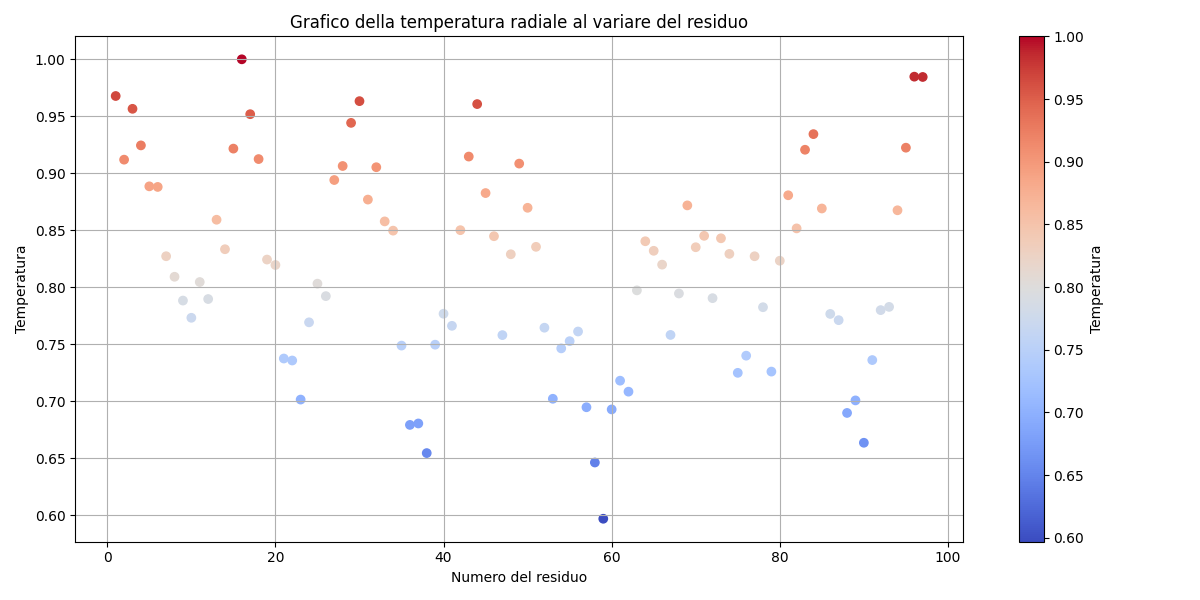
\includegraphics[width=0.5\textwidth]{"images/2m10_2_temperature_sferic.png"}
    \caption{Temperatura Radiale}
\end{figure}
\begin{figure}[H]
    \centering
    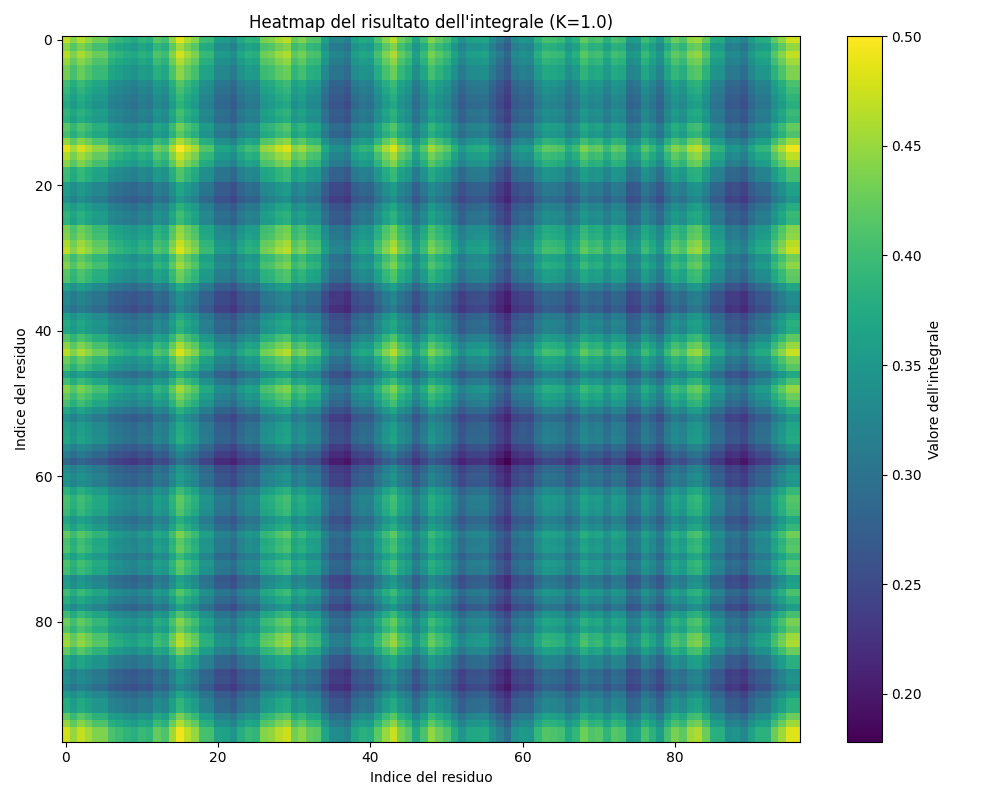
\includegraphics[width=0.5\textwidth]{"images/2m10_2_temperature_correlation_sferic.png"}
    \caption{Correlazione Radiale}
\end{figure}






\section*{Risoluzione dell'equazione differenziale e calcolo della correlazione}

Partiamo dall'equazione differenziale data per \( x_i(t) \):

\[
\frac{dx_i}{dt} = -\sum_j K_{ij} x_j + \sqrt{2 k_B T} \, \eta_i + \left(1 - \cos(\omega t)\right)(\delta_{a_i} - \delta_{b_i})
\]

dove:
- \( K_{ij} \) rappresenta la matrice di accoppiamento tra i nodi,
- \( \eta_i \) è un processo di Wiener (rumore bianco gaussiano) con \(\langle \eta_i(t) \eta_j(s) \rangle = \delta_{ij} \delta(t - s)\),
- \( \delta_{a_i} \) e \( \delta_{b_i} \) sono costanti di offset che definiscono la parte oscillatoria del sistema.

### Passaggio agli autovettori

Definiamo il cambiamento di base usando gli autovettori della matrice \( K \), scrivendo:

\[
x_i(t) = \sum_k V_{ik} Q_k(t)
\]

dove \( V \) è la matrice degli autovettori di \( K \), e \( Q_k(t) \) rappresenta la dinamica lungo ciascun autovettore. L'equazione differenziale per \( Q_k(t) \) diventa:

\[
\frac{dQ_k}{dt} = -\lambda_k Q_k + C_k (1 - \cos(\omega t)) + \sqrt{2 k_B T} \, \tilde{\eta}_k
\]

con:
- \( \lambda_k \) autovalori associati agli autovettori di \( K \),
- \( C_k = \sum_i V_{ik} (\delta_{a_i} - \delta_{b_i}) \),
- \( \tilde{\eta}_k = \sum_i V_{ik} \eta_i \) è il rumore proiettato sugli autovettori.

### Soluzione dell'equazione differenziale per \( Q_k(t) \)

La soluzione formale per \( Q_k(t) \) è data dalla somma di una parte deterministica e di una parte stocastica:

\[
Q_k(t) = Q_k^{\text{det}}(t) + Q_k^{\text{rumore}}(t)
\]

1. **Parte deterministica**: Integrando la parte deterministica, otteniamo

   \[
   Q_k^{\text{det}}(t) = C_k \left( \frac{1 - e^{-\lambda_k t}}{\lambda_k} - \frac{e^{-\lambda_k t} - \cos(\omega t) + \frac{\lambda_k}{\omega} \sin(\omega t)}{\lambda_k^2 + \omega^2} \right)
   \]

2. **Parte stocastica**: La soluzione per la parte stocastica dovuta al rumore è

   \[
   Q_k^{\text{rumore}}(t) = \sqrt{2 k_B T} \int_0^t e^{-\lambda_k (t - u)} \tilde{\eta}_k(u) \, du
   \]

   ### Calcolo della correlazione \(\langle x_i(t) x_j(s) \rangle\)

   La correlazione media \(\langle x_i(t) x_j(s) \rangle\) è:
   
   \[
   \langle x_i(t) x_j(s) \rangle = \sum_{k, l} V_{ik} V_{jl} \langle Q_k(t) Q_l(s) \rangle,
   \]
   
   dove \(\langle Q_k(t) Q_l(s) \rangle\) può essere suddivisa nei contributi deterministico e stocastico:
   
   \[
   \langle Q_k(t) Q_l(s) \rangle = \langle Q_k^{\text{det}}(t) Q_l^{\text{det}}(s) \rangle + \langle Q_k^{\text{rumore}}(t) Q_l^{\text{rumore}}(s) \rangle.
   \]
   
   #### Contributo deterministico
   
   La correlazione tra le parti deterministiche è:
   
   \[
   \langle Q_k^{\text{det}}(t) Q_k^{\text{det}}(s) \rangle = C_k^2 \left( f_k(t, s) + g_k(t, s) \cos(\omega (t - s)) + h_k(t, s) \sin(\omega (t - s)) \right),
   \]
   
   dove:
   - \( f_k(t, s) \) rappresenta il termine di decadimento esponenziale dato da:
     \[
     f_k(t, s) = \frac{(1 - e^{-\lambda_k t})(1 - e^{-\lambda_k s})}{\lambda_k^2},
     \]
   - \( g_k(t, s) \) rappresenta il termine di correlazione coseno:
     \[
     g_k(t, s) = \frac{e^{-\lambda_k(t+s)} - \cos(\omega t) \cos(\omega s)}{\lambda_k^2 + \omega^2},
     \]
   - \( h_k(t, s) \) rappresenta il termine di correlazione seno:
     \[
     h_k(t, s) = \frac{\lambda_k (\sin(\omega t) \cos(\omega s) + \cos(\omega t) \sin(\omega s))}{\lambda_k^2 + \omega^2}.
     \]
   
   #### Contributo stocastico
   
   Per la parte stocastica, otteniamo:
   
   \[
   \langle Q_k^{\text{rumore}}(t) Q_k^{\text{rumore}}(s) \rangle = \frac{k_B T}{\lambda_k} \delta_{kl} e^{-\lambda_k |t - s|}.
   \]
   
   ### Risultato finale
   
   Combinando i termini, otteniamo la correlazione media finale per \(\langle x_i(t) x_j(s) \rangle\):
   
   \[
   \langle x_i(t) x_j(s) \rangle = \sum_k V_{ik} V_{jk} \left( C_k^2 \left( f_k(t, s) + g_k(t, s) \cos(\omega (t - s)) + h_k(t, s) \sin(\omega (t - s)) \right) + \frac{k_B T}{\lambda_k} e^{-\lambda_k |t - s|} \right).
   \]
   
   Ogni termine è ora chiaramente identificato:
   - \( C_k^2 f_k(t, s) \): componente di decadimento esponenziale,
   - \( C_k^2 g_k(t, s) \cos(\omega (t - s)) \): componente oscillatoria con coseno,
   - \( C_k^2 h_k(t, s) \sin(\omega (t - s)) \): componente oscillatoria con seno,
   - \( \frac{k_B T}{\lambda_k} e^{-\lambda_k |t - s|} \): contributo del rumore termico.
   

   
   

\section*{Produzione di Entropia}

La produzione di entropia \( S \) può essere calcolata utilizzando l'espressione data per la forza \( F \) e l'equazione differenziale associata al sistema.

\subsection*{Equazione Differenziale}

Consideriamo l'equazione differenziale:

\[
\frac{dx_i}{dt} = -\sum_j K_{ij} x_j + \sqrt{2 k_B T} \eta_i + (1 - \cos(\omega t)) (\delta_{a_i} - \delta_{b_i}).
\]

\subsection*{Espressione per \( F \)}

L'espressione per \( F \) è data da:

\[
F = \sum_j K_{ij} x_j + (1 - \cos(\omega t)) (\delta_{a_i} - \delta_{b_i}).
\]

\subsection*{Produzione di Entropia}

La produzione di entropia può essere espressa come:

\[
S = \frac{F \cdot \frac{dx}{dt}}{T}.
\]

Sostituendo \( F \) e \( \frac{dx}{dt} \), otteniamo:

1. Sostituendo \( F \):

\[
F = \sum_j K_{ij} x_j + (1 - \cos(\omega t)) (\delta_{a_i} - \delta_{b_i}).
\]

2. Sostituendo \( \frac{dx}{dt} \):

\[
\frac{dx_i}{dt} = -\sum_k K_{ik} x_k + \sqrt{2 k_B T} \eta_i + (1 - \cos(\omega t)) (\delta_{a_i} - \delta_{b_i}).
\]

\subsection*{Produzione di Entropia Completa}

Pertanto, la produzione di entropia può essere scritta come:


\[
S = \frac{1}{T} \left[ \sum_j K_{ij} x_j \left( -\sum_k K_{ik} x_k + \sqrt{2 k_B T} \eta_i + (1 - \cos(\omega t)) (\delta_{a_i} - \delta_{b_i}) \right) + (1 - \cos(\omega t)) (\delta_{a_i} - \delta_{b_i}) \left( -\sum_k K_{ik} x_k + \sqrt{2 k_B T} \eta_i + (1 - \cos(\omega t)) (\delta_{a_i} - \delta_{b_i}) \right) \right].
\]


\subsection*{Considerazioni sulle Semplificazioni}

Esploriamo ora alcune possibili semplificazioni dell'espressione per la produzione di entropia:

\begin{enumerate}
    \item \textbf{Condizioni di Equilibrio}: Se il sistema è in equilibrio termico, potremmo avere \( \langle x_j \rangle \) costante, semplificando il calcolo della somma sui termini di \( K_{ij} x_j \).
    
    \item \textbf{Media Temporale}: Considerando la media temporale di \( S \), alcuni termini oscillatori (come quelli con \( \cos(\omega t) \)) potrebbero cancellarsi nel lungo termine, specialmente se le oscillazioni sono simmetriche attorno a zero.
    
    \item \textbf{Domini di Oscillazione}: Se i contributi oscillatori non sono dominanti, potremmo trascurarli per un'analisi qualitativa.
    
    \item \textbf{Assunzione di Piccole Oscillazioni}: Se le oscillazioni sono piccole, possiamo linearizzare i termini, ma questa assunzione potrebbe non essere sempre valida a seconda dell'ampiezza delle oscillazioni.
\end{enumerate}

\subsection*{Conclusioni}

In generale, mentre l'espressione per la produzione di entropia è complessa, alcune semplificazioni possono essere applicabili in condizioni specifiche, come stati di equilibrio o considerando medie temporali. Tuttavia, senza ulteriori informazioni sulle dinamiche del sistema o sul comportamento dei termini, non è facile ottenere una forma significativamente più semplice dell'espressione.




\section{Fokker planck N temperature}

L'equazione di Fokker-Planck associata all'equazione differenziale

\[
\frac{dx_i}{dt} = -\sum_j K_{ij} x_j + B \eta_i
\]

è data da:

\[
\frac{\partial P(x,t)}{\partial t} = \sum_i \frac{\partial}{\partial x_i} \left[ \sum_j K_{ij} x_j P \right] + \frac{1}{2} \sum_{i,j} \frac{\partial^2}{\partial x_i \partial x_j} \left[ B_{ii} \delta_{ij} P \right]
\]

dove:
\begin{itemize}
    \item \( P(x,t) \) è la densità di probabilità del sistema,
    \item \( A_i = -\sum_j K_{ij} x_j \) è il termine drift,
    \item \( D_{ij} = B_{ii} \delta_{ij} \) è la matrice di diffusione.
\end{itemize}





\section*{Soluzione dell'Equazione Differenziale}

Consideriamo l'equazione differenziale iniziale:

\[
\frac{\partial P}{\partial t} = \sum_i \left( \sum_j K_{ij} x_j P \right) + 0.5 \sum_{i,j} \left( \frac{\partial^2}{\partial x_i \partial x_j} (B_{ij} P) \right).
\]

Dove \( P = P(x, t) \), \( K \) è la matrice di Kirchhoff e \( B \) è una matrice diagonale.

Supponiamo una condizione iniziale:

\[
P(x, 0) = \delta(x - x_0).
\]

\subsection*{Trasformata di Fourier}

Applicando la trasformata di Fourier rispetto a \( x \):

\[
P(k, t) = \int_{-\infty}^{+\infty} P(x, t) e^{-ikx} \, dx.
\]

La trasformata dell'equazione diventa:

\[
\frac{\partial P(k, t)}{\partial t} = \int_{-\infty}^{+\infty} \left( \sum_i \left( \sum_j K_{ij} x_j P \right) \right) e^{-ikx} \, dx + 0.5 \int_{-\infty}^{+\infty} \left( \sum_{i,j} \frac{\partial^2}{\partial x_i \partial x_j} (B_{ij} P) \right) e^{-ikx} \, dx.
\]

\subsection*{Primo Termine: Derivata e Trasformata}

Focalizziamoci sul primo termine:

\[
\frac{\partial P(k, t)}{\partial t} = \sum_i \left( K_{ii} P(k, t) \right) + \sum_{i,j} K_{ij} \left( \int_{-\infty}^{+\infty} x_j P(x, t) e^{-ikx} \, dx \right).
\]

Per il secondo termine, utilizziamo la proprietà della trasformata di Fourier per la derivata:

\[
\int_{-\infty}^{+\infty} \frac{\partial^2 P}{\partial x_i \partial x_j} e^{-ikx} \, dx = -k_i k_j P(k, t).
\]

Quindi, l'equazione diventa:

\[
\frac{\partial P(k, t)}{\partial t} = \sum_i K_{ii} P(k, t) + \sum_{i,j} K_{ij} \left( -i \frac{\partial P(k, t)}{\partial k} \right) - 0.5 \sum_{i,j} B_{ij} k_i k_j P(k, t).
\]

\subsection*{Semplificazione}

Riorganizzando l'equazione, otteniamo:

\[
\frac{\partial P(k, t)}{\partial t} = \sum_i K_{ii} P(k, t) + \sum_{i,j} K_{ij} \left( -ik_j P(k, t) \right) - 0.5 \sum_{i,j} B_{ij} k_i k_j P(k, t).
\]

Definiamo \(\Lambda(k)\):

\[
\Lambda(k) = \sum_i K_{ii} + \sum_{i,j} K_{ij} (-ik_j) - 0.5 \sum_{i,j} B_{ij} k_i k_j.
\]

Quindi, l'equazione diventa:

\[
\frac{\partial P(k, t)}{\partial t} = \Lambda(k) P(k, t).
\]

\subsection*{Risoluzione dell'Equazione Differenziale}

La soluzione dell'equazione differenziale è:

\[
P(k, t) = P(k, 0) e^{\Lambda(k) t}.
\]

Utilizzando la condizione iniziale \( P(k, 0) = e^{-ikx_0} \):

\[
P(k, t) = e^{-ikx_0} e^{\Lambda(k) t}.
\]

\subsection*{Trasformata Inversa}

Per trovare \( P(x, t) \), applichiamo la trasformata di Fourier inversa:

\[
P(x, t) = \int_{-\infty}^{+\infty} P(k, t) e^{ikx} \, dk.
\]

Sostituendo \( P(k, t) \):

\[
P(x, t) = \int_{-\infty}^{+\infty} e^{-ikx_0} e^{\Lambda(k) t} e^{ikx} \, dk.
\]

Fattorizzando:

\[
P(x, t) = e^{-ix_0 k} \int_{-\infty}^{+\infty} e^{ik(x - x_0)} e^{\Lambda(k) t} \, dk.
\]

Assumiamo una forma specifica per \( \Lambda(k) \):

\[
\Lambda(k) = -\gamma k^2,
\]

dove \( \gamma \) è una costante positiva. Allora, otteniamo:

\[
P(x, t) = \int_{-\infty}^{+\infty} e^{ik(x - x_0)} e^{-\gamma k^2 t} \, dk.
\]

\subsection*{Risoluzione dell'Integrale}

Utilizziamo la formula dell'integrale gaussiano:

\[
P(x, t) = \sqrt{\frac{\pi}{\gamma t}} e^{-\frac{(x - x_0)^2}{4\gamma t}}.
\]

\subsection*{Risultato Finale}

La soluzione finale è:

\[
P(x, t) = \sqrt{\frac{\pi}{\gamma t}} e^{-\frac{(x - x_0)^2}{4\gamma t}}.
\]
\chapter{Conclusions}

\newpage
\null
\thispagestyle{empty}
\newpage
\addcontentsline{toc}{chapter}{\bibname}

\begin{thebibliography}{50}
%bibliografia
\end{thebibliography}

%\bibliographystyle{sapthesis} % BibTeX style
%\bibliography{bibliography} % BibTeX database without .bib extension

\end{document}
